\documentclass[11pt,a4paper]{article}

\usepackage[margin=1in]{geometry} 
\usepackage{graphicx}            


\usepackage[dvipsnames]{xcolor} % Gives you access to better color names
\usepackage{hyperref}

\hypersetup{
    colorlinks=true,      % Turns off the boxes, turns on colored text
    linkcolor=RoyalBlue,  % Color for internal links (Figs, Tabs, Equations, TOC)
    citecolor=ForestGreen, % Color for bibliographical citations
    urlcolor=Bittersweet, % Color for external web links
    filecolor=magenta,    % Color for local file links
    pdfpagemode=FullScreen,
}

\usepackage{listings}
\usepackage{gensymb}
\usepackage{svg}
\usepackage{fancyvrb} 
\usepackage{rotating} 
\usepackage{microtype}
\usepackage[title]{appendix}
\usepackage{float}
\usepackage[square]{natbib}
\usepackage{longtable} % Added here in the preamble where it belongs
\usepackage{caption} 
% \usepackage{draftwatermark}
\usepackage{fancyhdr}
\usepackage{graphicx}
% \usepackage{lineno}

\usepackage{fancyhdr}
\usepackage{lastpage} 

% --- Watermark Configuration ---
% \usepackage{draftwatermark}
% \SetWatermarkText{DRAFT}
% \SetWatermarkScale{6}   % <-- Increase this from 5 to 12 (or higher if needed)
% \SetWatermarkColor[gray]{0.85} % <-- Slightly darker gray for better visibility
% -------------------------------
 

% --- Global Page Style Setup --- 
\pagestyle{fancy}
\fancyhf{} % Clear everything once

% --- Header Setup ---
\rhead{
\includegraphics[width=4cm]{NCAS_logo_transparent.png}} 

\renewcommand{\headrulewidth}{0.4pt} % Optional: adds a thin line under the logo



% Place the logo in the top right (R) header (H)
\rhead{
\includegraphics[width=4cm]{NCAS_logo_transparent}} 



% Optional: Remove the horizontal line under the header
% \renewcommand{\headrulewidth}{0pt}



% \captionsetup[table]{skip=10pt} % Adjust the 10pt to your liking

% \hypersetup{
%     hidelinks
% }

\title{Climate and Forecasting Aggregation (CFA) file preparation for the CANARI climate model ensemble}

\author{
    Jonny Williams\thanks{\url{jonny.williams@ncas.ac.uk}}, David Hassell, Bryan Lawrence \\
    NCAS-CMS
}
\date{\today}

\begin{document}

\maketitle 
\thispagestyle{fancy}
\tableofcontents

\clearpage




\setcounter{section}{-1}

\section{Project structure}

Figure \ref{fig:project_structure} and Listing \ref{lst:project_structure} show the project structure and the code to generate it respectively.

\begin{figure}[H]
    \centering
    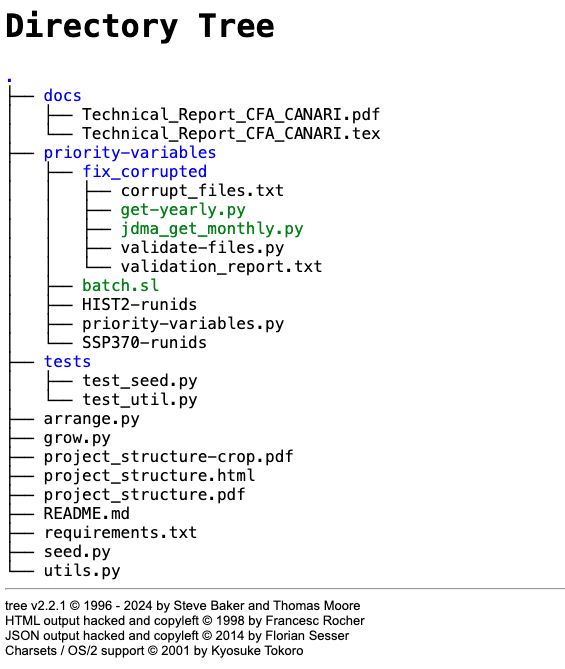
\includegraphics[width=0.8\textwidth]{figures/project_structure.png}
    \caption{}
    \label{fig:project_structure}
\end{figure}




\begin{center}
\begin{minipage}{\textwidth}
\begin{lstlisting}[
    basicstyle=\small\ttfamily,
    label={lst:project_structure},
    frame=single,
    backgroundcolor=\color{gray!5},
    breaklines=true,caption={\texttt{tree$\ldots$} command run in base of repository.},
    keepspaces=true,
    columns=fullflexible
]
tree -F --dirsfirst --noreport -C -I 'CFA-files|HIST2|SSP370|u-*|_*|*.cfa|plantUML|figures|bib*|*png|go|*.aux|*.bbl|*.blg|*.fdb_latexmk|*.fls|*.log|*.out|*.synctex.gz|*.toc' -H . -o project_structure.html
\end{lstlisting}
\end{minipage}
\end{center}



\clearpage

\section{Introduction}

This document details the processes by which data from the CANARI project -- large ensembles of simulations using the HadGEM3-GC3.1 climate model \citep{williams2018} -- has been aggregated after its ingestion into the Joint-storage Data Migration App \label{jdma} (JDMA) archive\footnote{\url{https://help.jasmin.ac.uk/docs/short-term-project-storage/jdma/}}. The JDMA archive is hosted on the JASMIN platform hosted by the Centre for Environmental Data Analysis, CEDA\footnote{\url{https://www.ceda.ac.uk}}.

The CANARI ensemble consists of two, 40-member ensembles:

\begin{enumerate}
    \item Historical simulations running from 
1850-2015.\label{simlen}
\item SSP3-7.0 future scenarios, 2015-2100.
\end{enumerate}

SSP stands for Shared Socioeconomic Pathway. These are a family of potential future greenhouse gas and land-use pathways which are standardised and extensively used in the climate science community, more information can be found in \citet{ipcc2023syr}. 

Within the respective ensembles, each member differs only in its initial conditions, which are generated using a hybrid `macro-micro` initialisation method \citep{schiemann2026}.

Each simulation generates data in three month `batches' and the format of the batches' contents are described as, e.g., \texttt{runid/cyclepoint}, where \texttt{runid} takes the form \texttt{u-ab123} and \texttt{cyclepoint} is in the ISO-8601 `datetime' standard, e.g. \texttt{19500101T0000Z} \citep{iso8601}. Each batch is then given an integer index which describes its `location' on the JDMA archive. These values are given on the NCAS-CMS GitHub pages\footnote{\url{https://ncas-cms.github.io/canari}} and an example is given in Figure \ref{fig:batches}\label{batches}. The data is held in monthly files and so each batch contains three sets of data in a common format.





\begin{figure}[H]
    \centering
    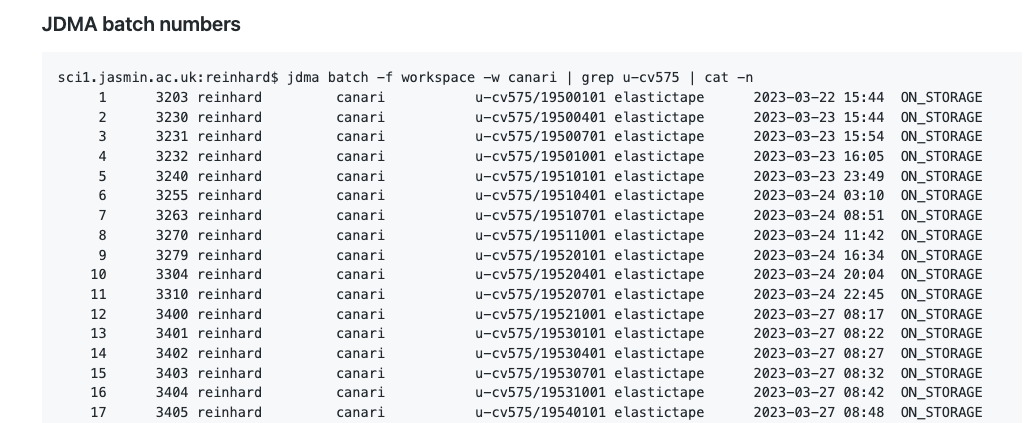
\includegraphics[width=\textwidth]{figures/batches.png}
    \caption{Example of JDMA batch indexing from the CANARI project pages.}
    \label{fig:batches}
\end{figure}

\section{Workflow}

The workflow discussed here assumes that the diagnostic content of each simulation is the same. In almost every respect this is the case, except for four variables in the atmospheric output in the historical simulations; this will be discussed in \S~\ref{note}. This assumption significantly reduces the time taken to generate the `seed' files described below which make up the vast majority of the processing time. Table \ref{tab:runids} shows the simulation identifiers for the historical and SSP3-7.0 simulations. Their format is standard for climate models run with the Rose and Cylc \citep{Oliver2018} workflow tools. Rose is `a framework for managing and running meteorological suites'\footnote{\url{https://www.metoffice.gov.uk/research/approach/modelling-systems/rose}} and Cylc is `a general purpose workflow engine with a particular gift for cycling'\footnote{\url{https://cylc.github.io}}.

 
\subsection{Aggregation with \texttt{cf} Python}

CF aggregation is a new feature in the CF conventions, having been available since December 2025 \citep{eaton_2025_17801666}. Their usage in this particular application is in the representation of a large database of climate model data -- $\mathcal{O}(\mathrm{PB})$ -- in a format which is portable and easily reproducible -- $\mathcal{O}({100\mathrm{MB}})$ or less. The workflow must also be achievable in a timescale which enables easy reruns and big fixes, $\mathcal{O}(1~\mathrm{day})$ or less.

\begin{table}
\centering


\renewcommand{\arraystretch}{1.1} % Adds a tiny bit of breathing room between rows
\begin{tabular}{r l l | r l l}
% No \hline at the top
\textbf{ID} & \textbf{Historical} & \textbf{SSP3-7.0} & \textbf{ID} & \textbf{Historical} & \textbf{SSP3-7.0} \\ \hline
1  & \texttt{\colorbox{blue!20}{u-cv575}}~$^*$ & \texttt{\colorbox{blue!20}{u-de814}} & 21 & \texttt{u-da179} & \texttt{u-df933} \\
2  & \texttt{u-cv625}~$^*$ & \texttt{u-de436} & 22 & \texttt{u-da190} & \texttt{u-df934} \\
3  & \texttt{u-cw345}~$^*$ & \texttt{u-de724} & 23 & \texttt{u-da191} & \texttt{u-df935} \\
4  & \texttt{u-cw356}~$^*$ & \texttt{u-de815} & 24 & \texttt{u-da192} & \texttt{u-df936} \\
5  & \texttt{u-cv827}~$^*$ & \texttt{u-df220} & 25 & \texttt{u-da193} & \texttt{u-df937} \\
6  & \texttt{u-cv976}~$^*$ & \texttt{u-de830} & 26 & \texttt{u-db291} & \texttt{u-dh412} \\
7  & \texttt{u-cz547}~$^*$ & \texttt{u-de831} & 27 & \texttt{u-db301} & \texttt{u-dh413} \\
8  & \texttt{u-cy436}~$^*$ & \texttt{u-de832} & 28 & \texttt{u-db303} & \texttt{u-dh415} \\
9  & \texttt{u-cw342}~$^*$ & \texttt{u-de850} & 29 & \texttt{u-db304} & \texttt{u-dh416} \\
10 & \texttt{u-cw343}~$^*$ & \texttt{u-de851} & 30 & \texttt{u-db305} & \texttt{u-dh417} \\
11 & \texttt{u-cy375}~$^*$ & \texttt{u-de934} & 31 & \texttt{u-cz475} & \texttt{u-di511} \\
12 & \texttt{u-cy376}~$^*$ & \texttt{u-de937} & 32 & \texttt{u-cz568} & \texttt{u-di512} \\
13 & \texttt{\colorbox{blue!20}{u-cy537}} & \texttt{u-de938} & 33 & \texttt{u-cz647} & \texttt{u-di513} \\
14 & \texttt{u-cy811} & \texttt{u-de939} & 34 & \texttt{u-cz648} & \texttt{u-di514} \\
15 & \texttt{u-cy866} & \texttt{u-de940} & 35 & \texttt{u-cz649} & \texttt{u-di515} \\
16 & \texttt{u-cy873} & \texttt{u-df299} & 36 & \texttt{u-dd436} & \texttt{u-di703} \\
17 & \texttt{u-cy877} & \texttt{u-df300} & 37 & \texttt{u-dd438} & \texttt{u-di704} \\
18 & \texttt{u-cy879} & \texttt{u-df301} & 38 & \texttt{u-dd439} & \texttt{u-di705} \\
19 & \texttt{u-cy880} & \texttt{u-df302} & 39 & \texttt{u-dd441} & \texttt{u-di706} \\
20 & \texttt{u-cy881} & \texttt{u-df303} & 40 & \texttt{u-dd442} & \texttt{u-di707} \\
\hline
\end{tabular}%\label{tab:runids}
\caption{Ensemble Member RunIDs for Control and SSP3-7.0 scenarios. The simulations marked with asterisks have a slightly different output variable set   and the ensemble members used as `seeds' are \colorbox{blue!20}{highlighted}; see \S~\ref{grow}.}
\label{tab:runids}
\vspace{10pt}
\end{table}  

\subsection{Workflow diagram}

After choosing the scenario and seed simulation ID, the workflow is made up of three stages; seed, grow and arrange. This is illustrated in Figure \ref{fig:wholewf}. The individual algorithms for the seed, grow and arrange steps are shown in Figure \ref{fig:seed}, \ref{fig:grow} and \ref{fig:arrange} respectively.

\begin{figure}
    \centering
    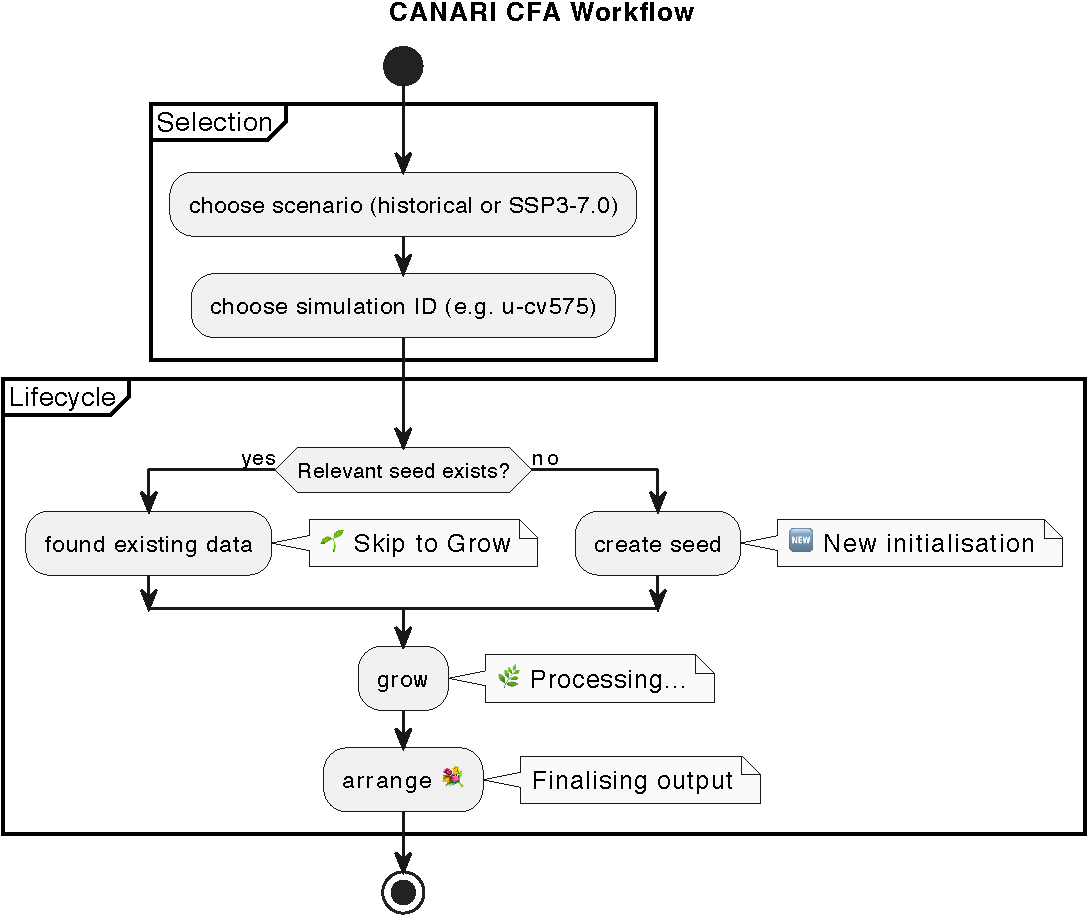
\includegraphics[width=\textwidth]{figures/wf-crop}
    \caption{Workflow diagram of the whole process of generating the CFA files, including choosing the scenario and simulation ID. Figure prepared using \texttt{PlantUML}.}
    \label{fig:wholewf}
\end{figure}


\subsection{Seed}\label{sseed}

The seed stage requires one complete month (only) of data on locally accessible disk. It is this month which is interrogated by the Python script \texttt{seed.py} and generates a seed file which is then `grown' -- \S~\ref{grow} -- and `arranged' -- \S~\ref{arrange} -- to give the final CFA file for the complete run length of the simulation (see page \pageref{simlen}). 

For example, the files which are used in the creation of the seed file for the historical ensemble are of the form \texttt{\detokenize{cv575{a,o,i}_1*195001*.nc}}, where \texttt{\detokenize{{a,o,i}}} uses the standard Linux wildcard syntax for `a or o or i' to refer to the atmosphere, ocean and sea ice datasets respectively. Going forward we use the term `realm' to refer to this distinction. This in turn assumes a consistent naming convention of the post processed ensemble data, and we assume this to be the case throughout the ensembles.

Of primary importance for the understanding of later sections of this document are the variables which describe the following:

\begin{itemize}
    \item File names
    \begin{itemize}
        \item These are called \texttt{\detokenize{fragment_uris}} in the language of the CF conventions\footnote{\url{https://cfconventions.org}} where \texttt{uris} are Uniform Resource Identifiers.
    \end{itemize}
    \item JDMA batch numbers
    \begin{itemize}
        \item These are called \texttt{\detokenize{fragment_unique_values}} in the CF conventions.
    \end{itemize}
    
\end{itemize}

Figure \ref{fig:frags} shows a screenshot of a section of the \texttt{ncdump} output from the resulting seed CFA file. The \texttt{\detokenize{fragment_unique_values}} and \texttt{\detokenize{fragment_uris}} variables are highlighted.   

\begin{figure}
    \centering
    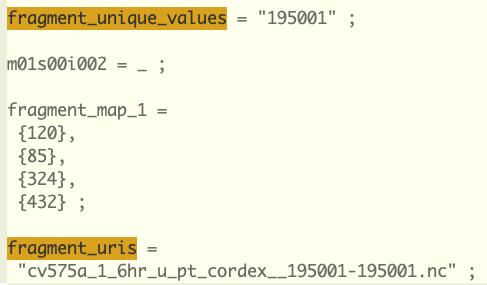
\includegraphics[width=\textwidth]{figures/frags.png}
    \caption{\texttt{\detokenize{fragment_unique_values}} and \texttt{\detokenize{fragment_unique_values}} variables in the historical simulations' seed CFA file.}
    \label{fig:frags}
\end{figure}

Note that in the seed file, the \texttt{\detokenize{fragment_unique_values}} string is set to the value of \texttt{year}$+$\texttt{month} strings in the \texttt{seed.py} file where \texttt{01} is January etc. This convention is also used in the \texttt{grow.py} described in \S~\ref{grow}.

The seed Python file also removes the NetCDF \texttt{name} attribute, which by default points to the original creation location on disk when the simulation was first run and is hence irrelevant -- and potentially misleading -- once the data has undergone any processing. The \texttt{seed.py} file must be run separately for each realm as is the case for the `grow' and `arrange' steps too.

Finally, Figure \ref{fig:seed} shows a visual representation of the algorithm used in \texttt{seed.py}.

\begin{figure}
    \centering
    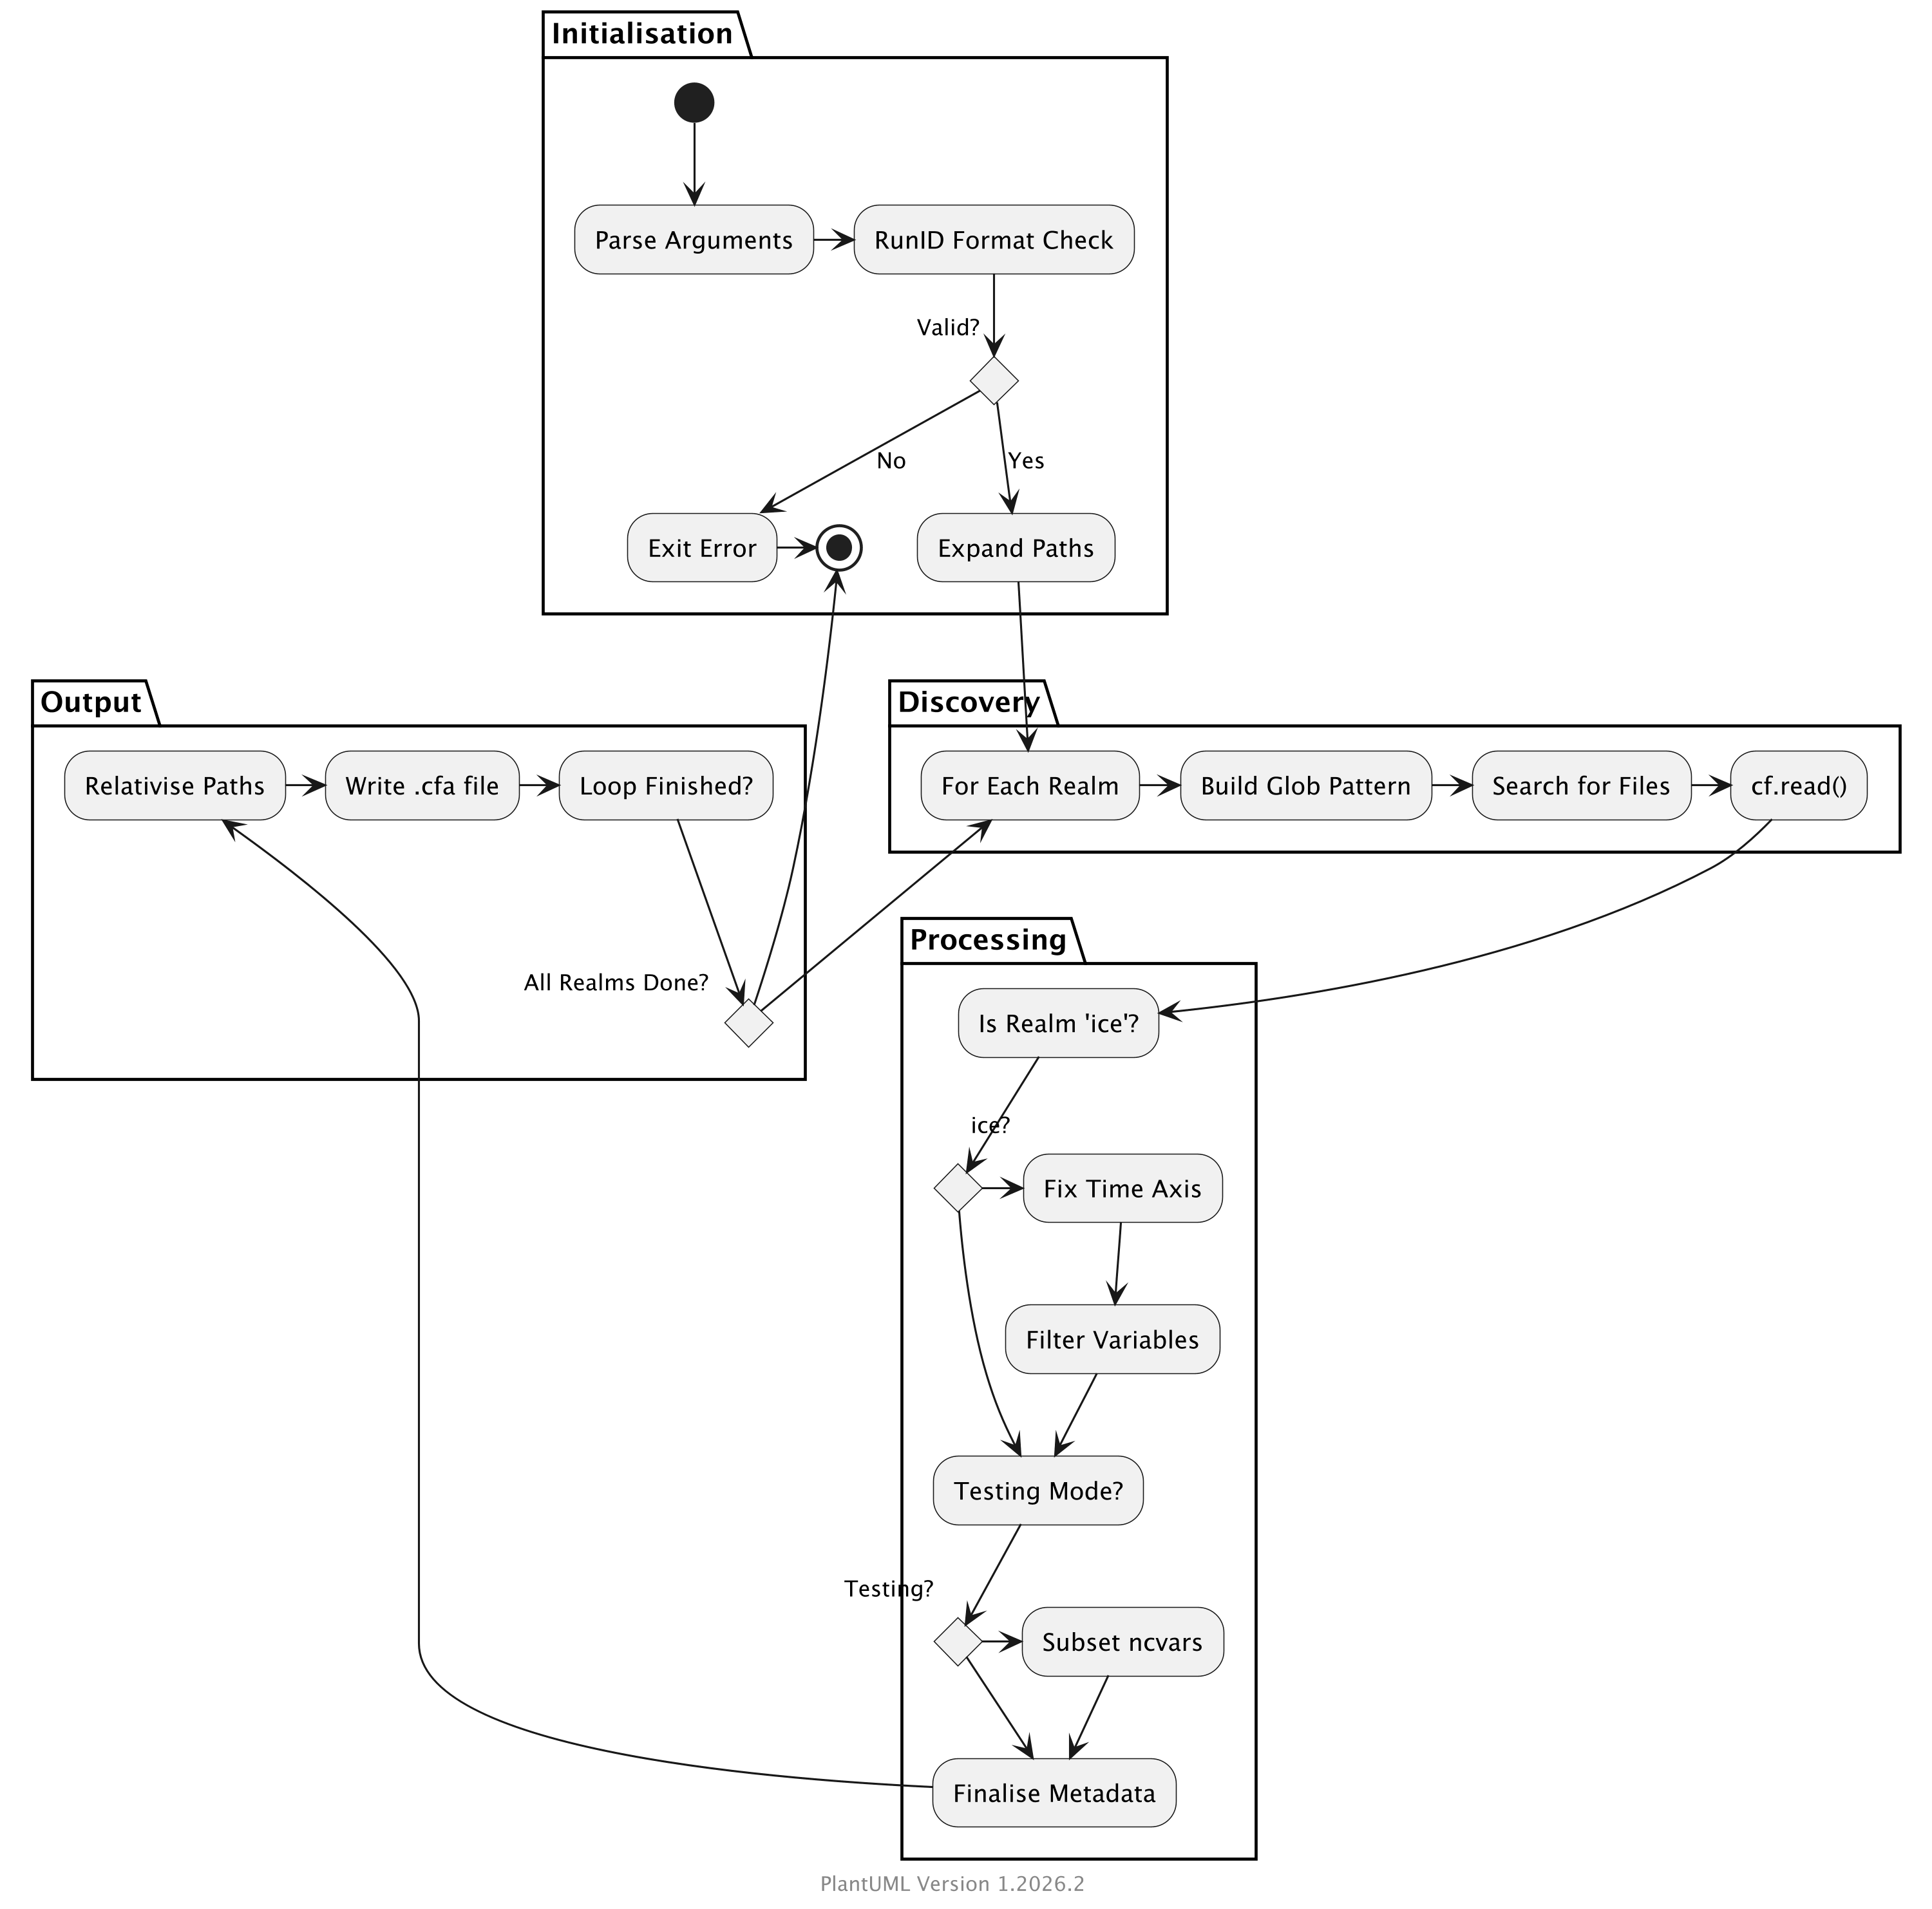
\includegraphics[width=0.8\textwidth]{figures/seed.png}
    \caption{Algorithm for the \texttt{seed.py} file, prepared with \texttt{PlantUML} \citep{plantuml}. }
    \label{fig:seed}
\end{figure}



\subsection{Grow}\label{grow}

Figure \ref{fig:grow} shows the \texttt{PlantUML} visualisation of the \texttt{grow.py} script. The majority of the code in this step of the overall workflow is concerned with the formatting of the date-time strings which, as part of the filenames -- i.e. \texttt{\detokenize{fragment_uris}} -- are grown, month by month, up to the end of the simulation's runtime (historical, 65 years; SSP3-7.0 85 years). 


\begin{figure}
    \centering
    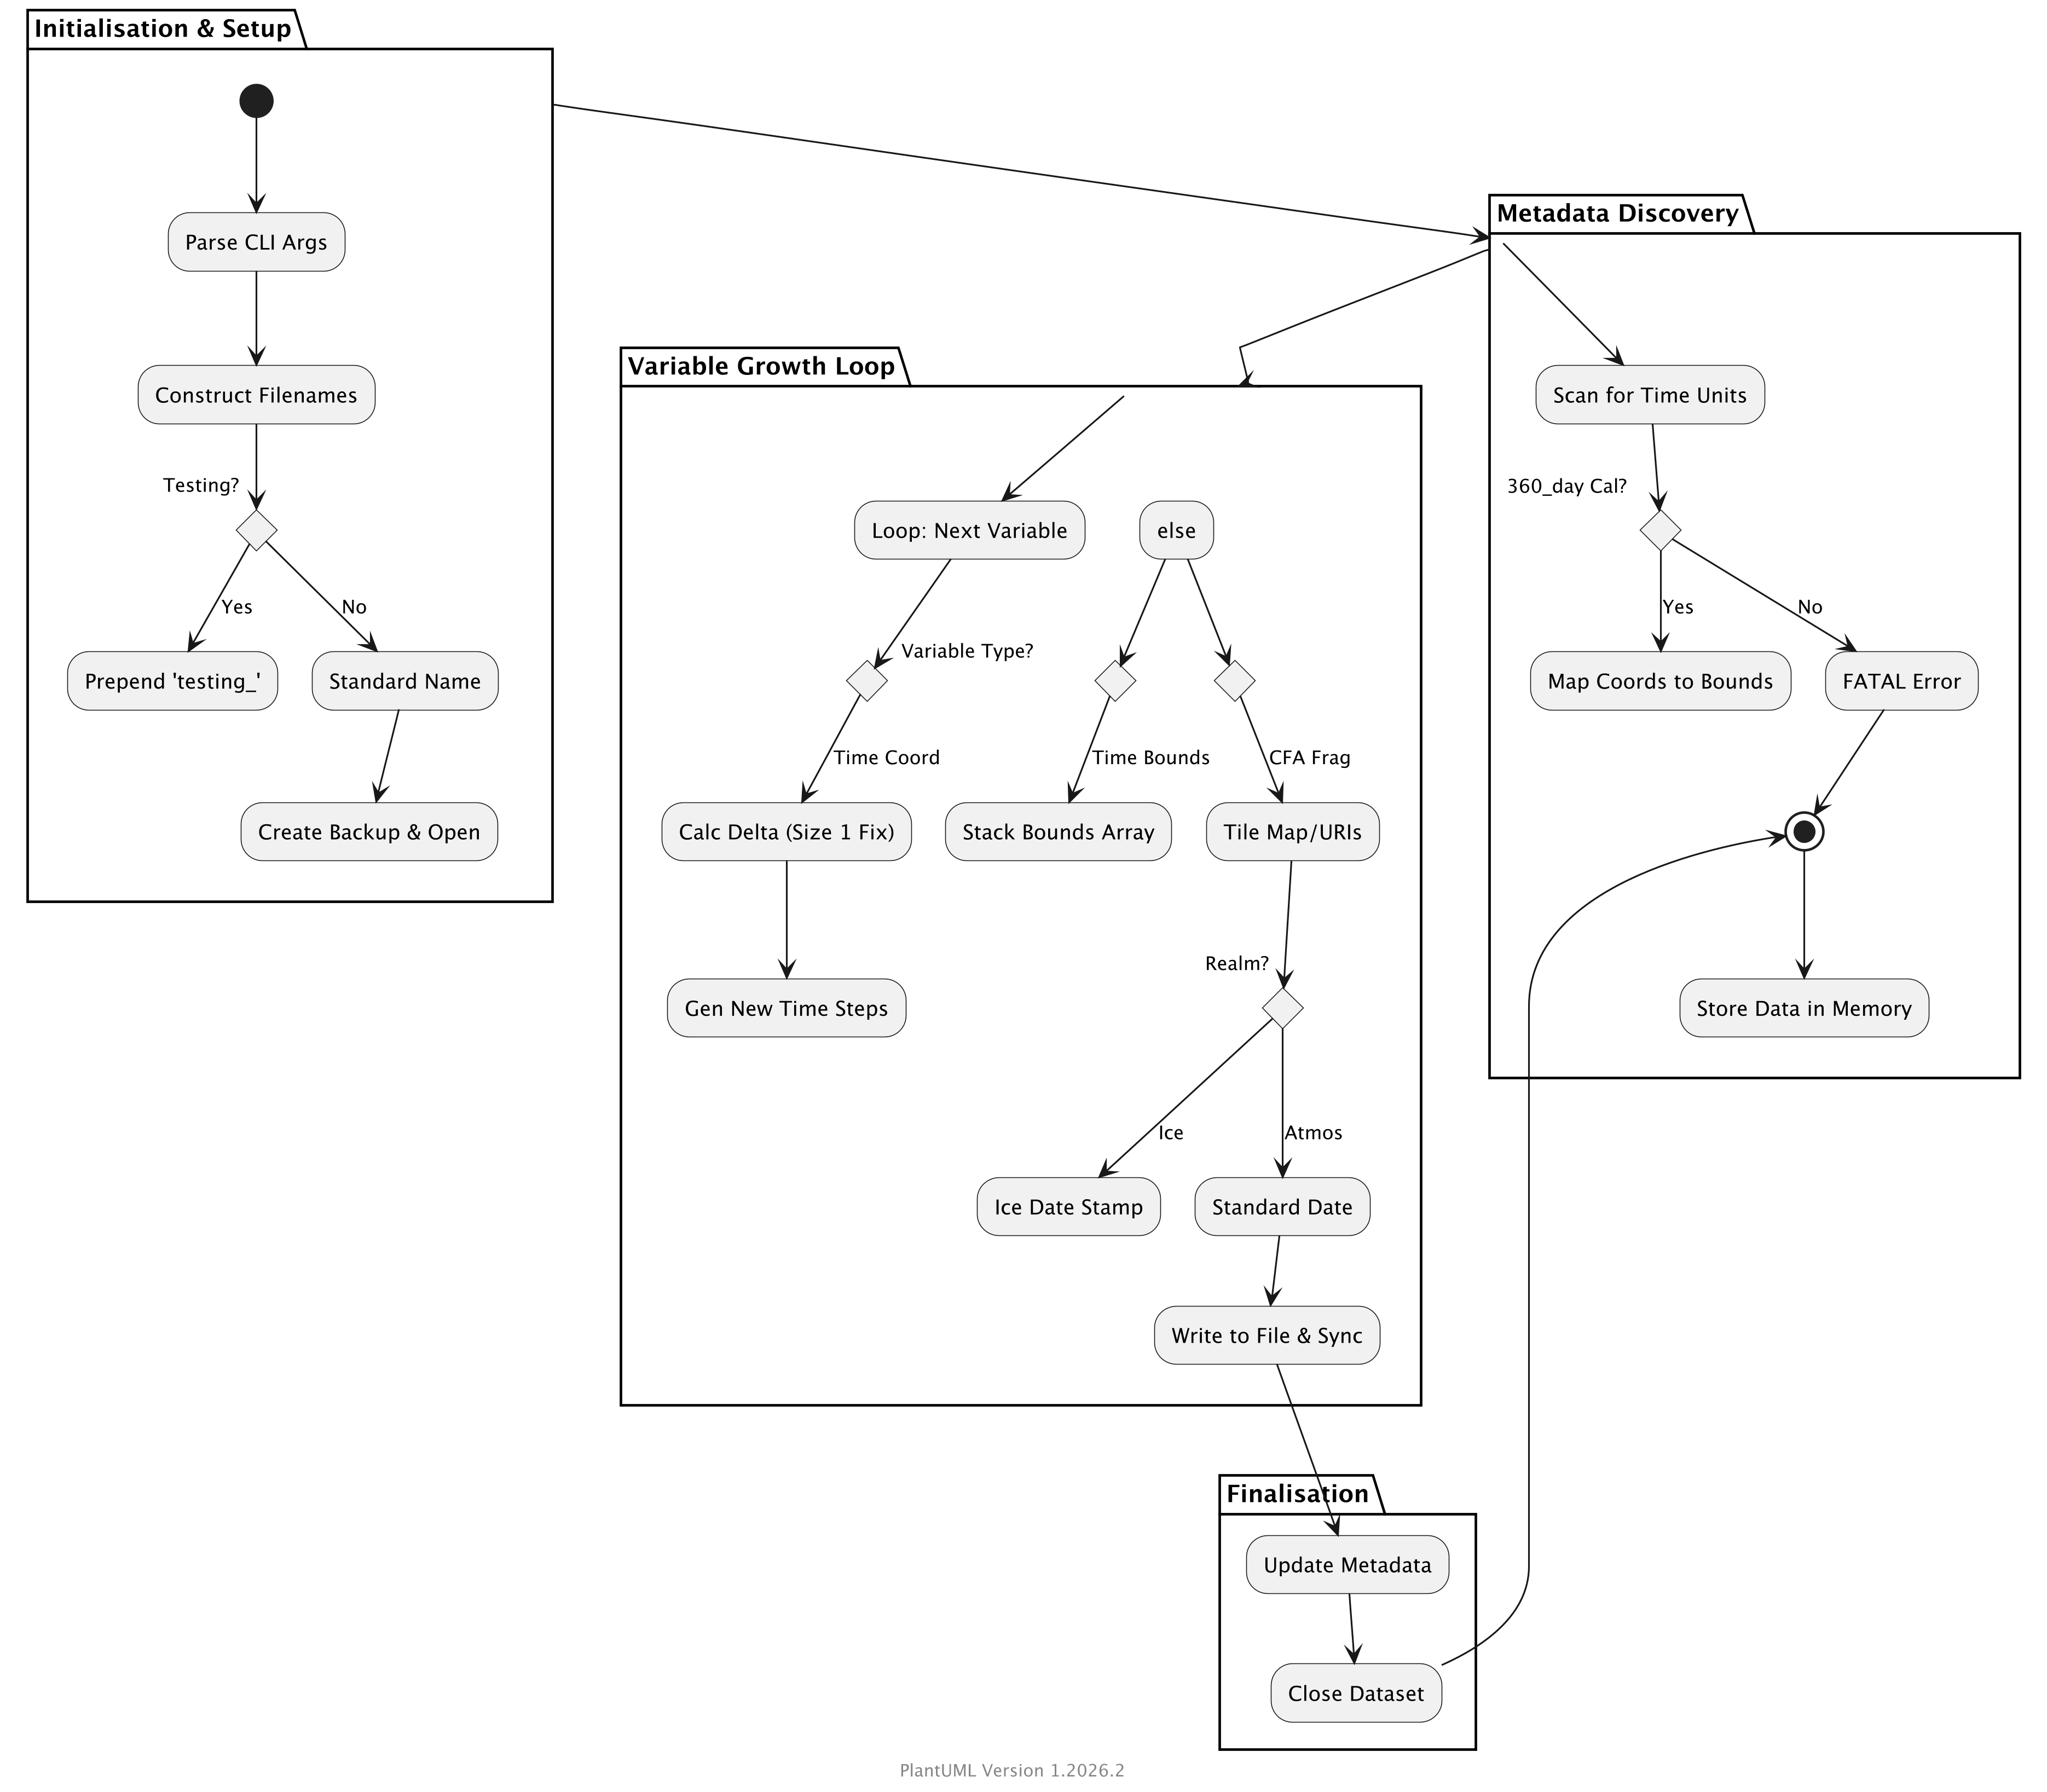
\includegraphics[width=\textwidth]{figures/grow.png}
    \caption{Algorithm for the \texttt{grow.py} file. }
    \label{fig:grow}
\end{figure}

Figure \ref{fig:grown} shows the first 14 months for the \texttt{\detokenize{fragment_uris}} variable\footnote{Note that this is the first of these, the \textit{second} is named \texttt{\detokenize{fragment_uris_1}} and so forth.}. The equivalent \texttt{\detokenize{fragment_unique_values}} variables are simply a reproduction -- to the same size as the \texttt{\detokenize{fragment_uris}} -- of that from the seeding step, i.e., placeholders of the form \texttt{195001} and \texttt{201501} for the historical and SSP3-7.0 ensembles respectively. The \texttt{arrange.py} edits these `dummy' values and is described in \S~\ref{arrange}.

The growth step is only required to be run for the `seed' simulations, i.e. the highlighted ones in Table \ref{tab:runids}. The arrangement step creates the final required files for the entire ensemble.  


\begin{figure}
    \centering
    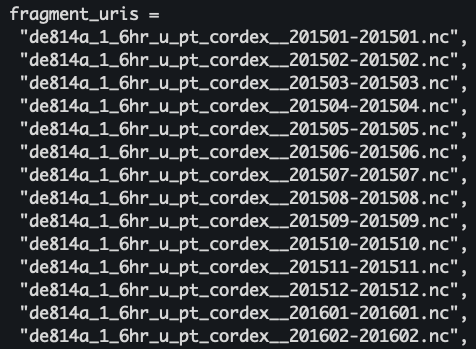
\includegraphics[width=\textwidth]{figures/grown.png}
    \caption{Example selection (first 14 months) \texttt{\detokenize{fragment_uris}} of the grown atmosphere CFA file for the first SSP3-7.0 ensemble member.}
    \label{fig:grown}
\end{figure}

\subsubsection{Note on historical diagnostic sets}\label{note}

For the historical ensemble, members 1-13 have slightly different variable sets\footnote{see \url{https://ncas-cms.github.io/canari/}} to the remainder. Therefore, members 2-12 were seeded from member 1, \texttt{u-dv575}, and 14-40 were seeded from member 13, \texttt{u-cy537}. All SSP3-7.0 members were seeded from its first member, \texttt{u-de814}.

\subsection{Arrange}\label{arrange} 
\subsubsection{JDMA batch IDs}
Figure \ref{arrange} shows the algorithm for the `arrangement' step. 

\begin{figure}
    \centering
    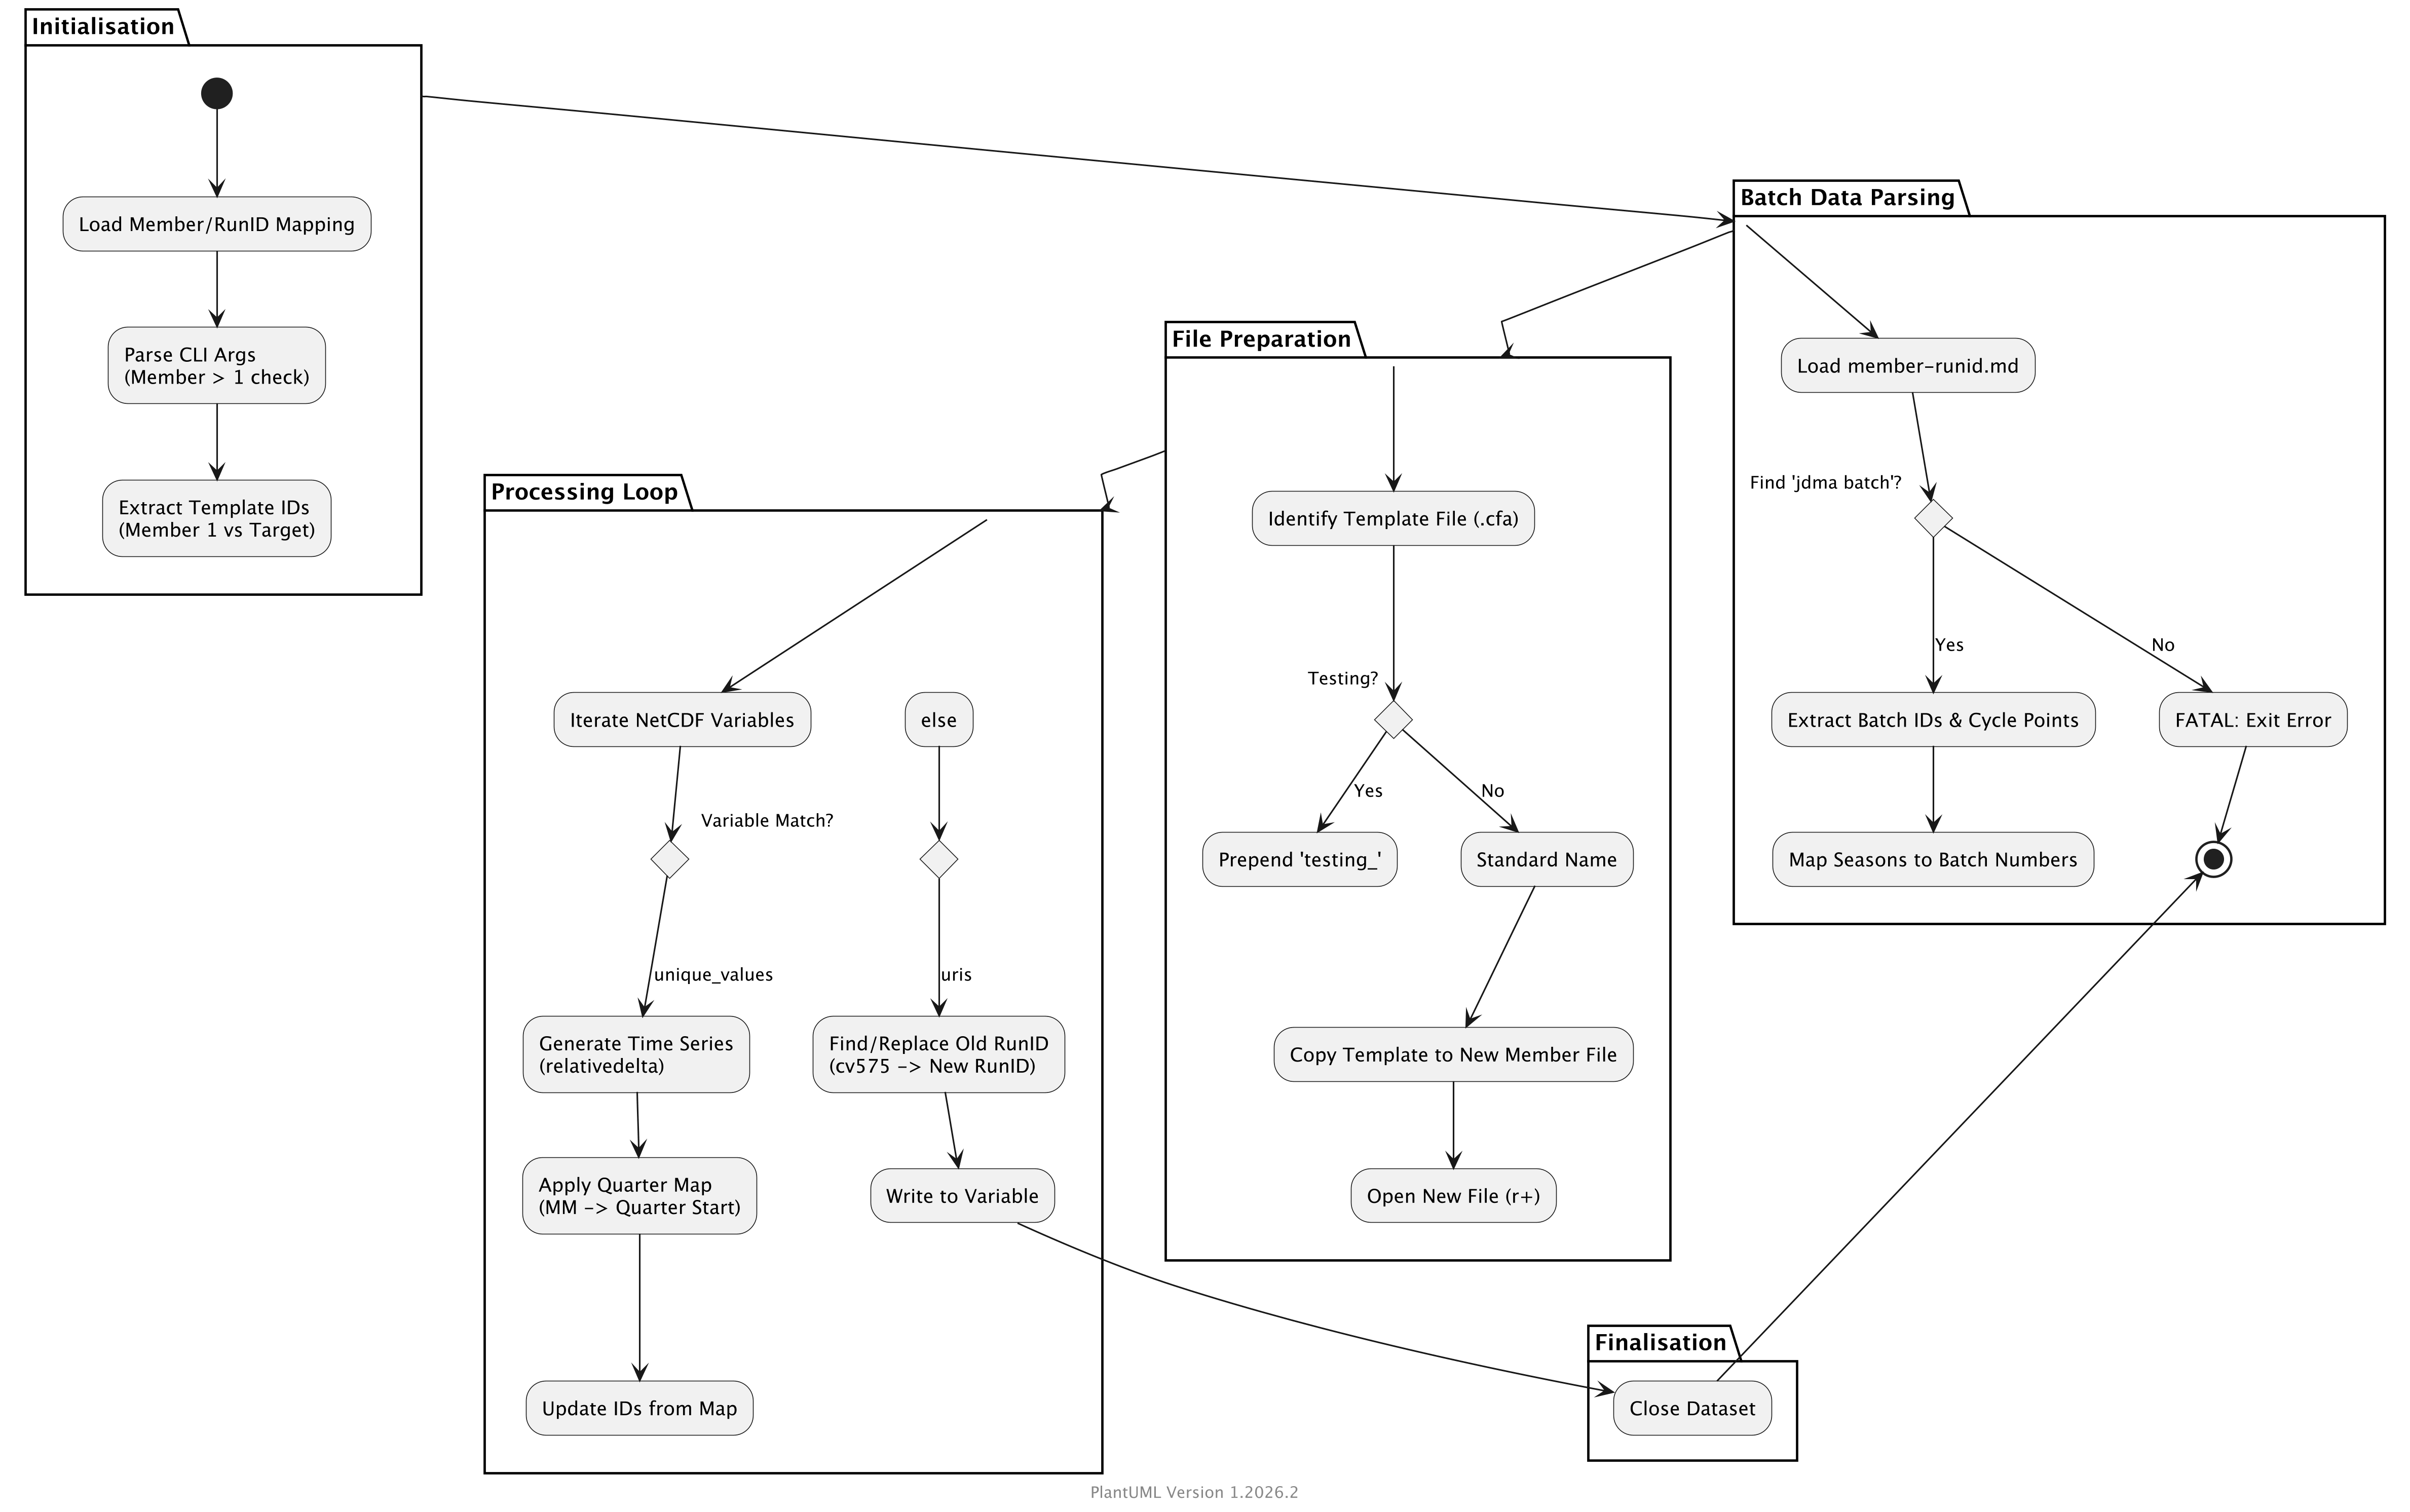
\includegraphics[width=\textwidth]{figures/arrange.png}
    \caption{Algorithm for the \texttt{arrange.py} file. }
    \label{fig:arrange}
\end{figure}

When the CANARI ensemble was run, the JDMA batch numbers associated with each three month cycle were manually documented -- see page \ref{batches} -- and these values are used as `lookup tables' to find the relevant batch number from the datetime string in the \texttt{\detokenize{fragment_uri}} values. An important step here is to convert the monthly -- \texttt{195001, 195002} -- datetime strings into the correct three-monthly cycle points. The need for this is illustrated in Figure \ref{fig:batches} where the batches are names \texttt{195001}, \texttt{195004}, etc. This is the `quarter map' step shown in Figure \ref{fig:arrange}.

\begin{sloppypar}

The results of the arrangement step is shown in Figure \ref{fig:uniquevalues}, which shows the \texttt{\detokenize{fragment_unique_values}} generated from the \texttt{arrange.py} script for the equivalent information shown in the CANARI online documentation in Figure \ref{fig:uniquevaluesvalidation}.

\end{sloppypar}


\begin{figure}
    \centering
    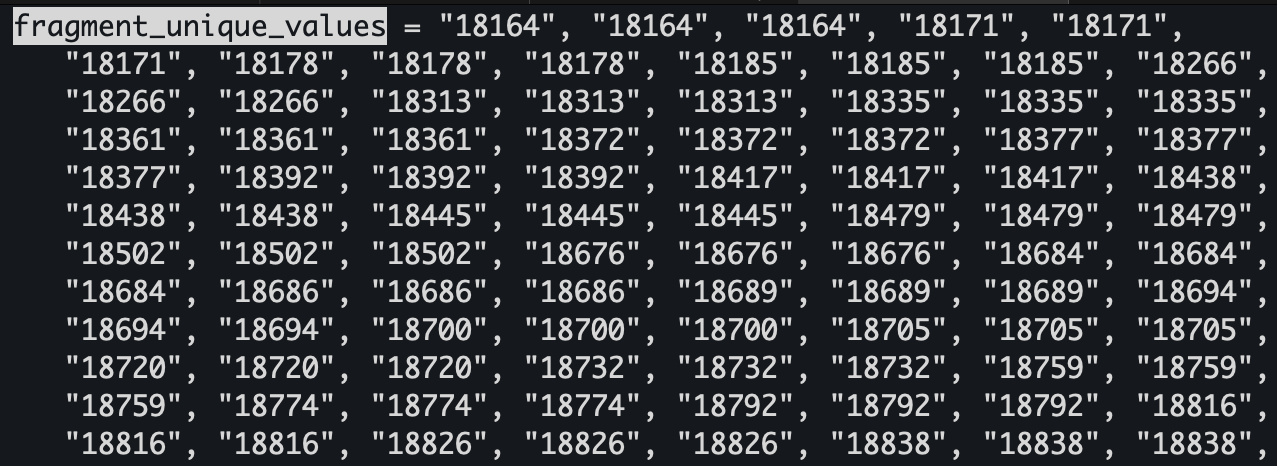
\includegraphics[width=\textwidth]{figures/uniquevalues}
    \caption{The \texttt{\detokenize{fragment_unique_values}} variable for the first several years of the simulation \texttt{u-de814}.}
    \label{fig:uniquevalues}
\end{figure}

\begin{figure}
    \centering
    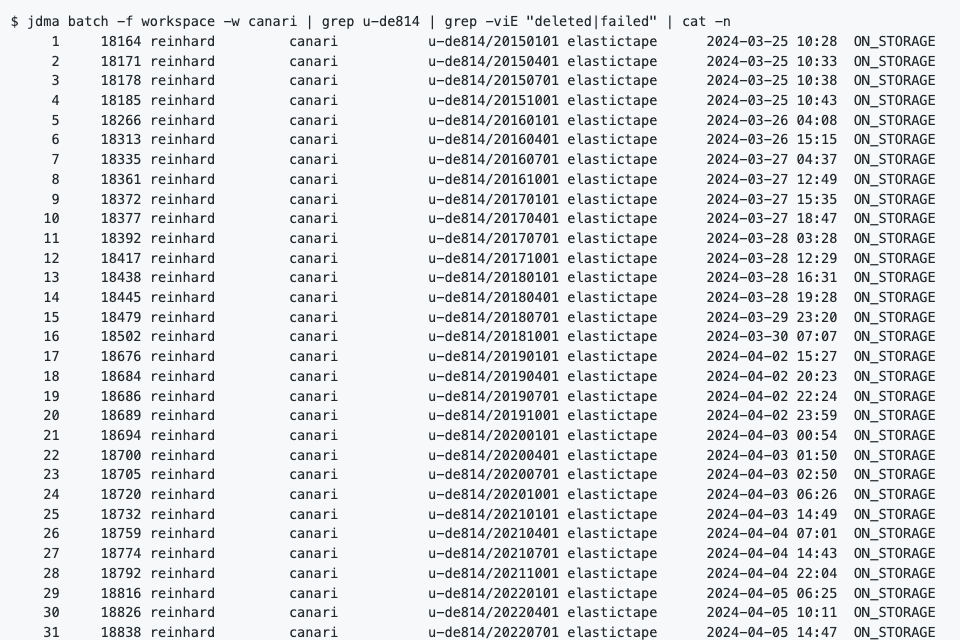
\includegraphics[width=\textwidth]{figures/uniquevaluesvalidation}
    \caption{The JDMA batch numbers variable for the first several years of the simulation \texttt{u-de814}. The period shown is the same as shown in Figure \ref{fig:uniquevalues}.}
    \label{fig:uniquevaluesvalidation}
\end{figure}

\subsubsection{JDMA `external' IDs}

Ongoing work will see the data on the JDMA archive moved to the Near-Line Data Store (NLDS).\footnote{\url{https://help.jasmin.ac.uk/docs/short-term-project-storage/nlds/}} To assist in this process, the elastic tape `external IDs' are also required. These numbers are found from the \texttt{jdma batch} command as shown in Listing \ref{lst:jdma-batch}):

\begin{center}
\begin{minipage}{\textwidth}
\begin{lstlisting}[
    basicstyle=\small\ttfamily,
    label={lst:jdma-batch},
    frame=single,
    backgroundcolor=\color{gray!5},
    breaklines=true,caption={\texttt{jdma batch} output},
    keepspaces=true,
    columns=fullflexible
]
jdma batch 3203
    Batch for user: pug123
    Batch id     : 3203 <--- Needed in CFA files!
    Workspace    : canari
    Batch label  : u-cv575/19500101T0000Z
    Ex. storage  : elastictape
    Date         : 2023-03-22 15:44
    External id  : 33076 <--- Needed in CFA files!
    Stage        : ON_STORAGE
\end{lstlisting}
\end{minipage}
\end{center}

\begin{sloppypar}
The final format of the \texttt{\detokenize{fragment_unique_values}} strings is, e.g., \texttt{\detokenize{3203_33076}}, i.e. \texttt{\detokenize{[batch_ID]_[external_ID]}}. 
\end{sloppypar}

\section{Example usage and validation}

Here we check that the output CFA files do indeed match the expected structure imposed on them by the method outlined above. 

\subsection{One day of 3-hourly, 1.5~m air temperature}\label{example}

Figure \ref{fig:CFAvalidation} shows code from a Jupyter notebook where the resulting CFA file for member 1 of the historical ensemble is opened using \texttt{cf.read}. After this, the 1.5~m temperature is read. This diagnostic appears many times in the output (on different time and spatial domains) and so we have then further concentrated on 3-hourly values, resulting in a single field. We then choose a random day in the 1950-2014 time series and examine the properties of the resulting 8 fields.

\begin{figure}
    \centering
    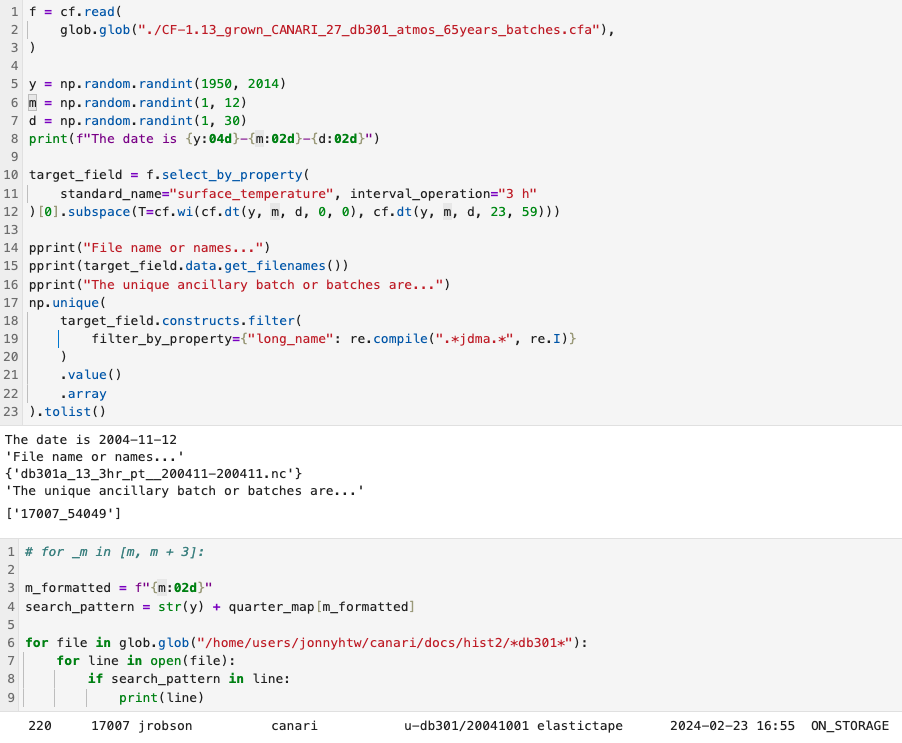
\includegraphics[width=\textwidth]{figures/CFAvalidation}
    \caption{Validation of one day of 3-hourly 1.5~m air temperature output; comparison of CFA file resulting from this work and the raw JDMA batch information.}
    \label{fig:CFAvalidation}
\end{figure}
 
\begin{sloppypar}
For this example, the date is 12/11/2004 and this is correctly identified with the file \texttt{\detokenize{db301a_13_3hr_pt__200411-200411.nc}}. The field's ancillary data are the JDMA batches which in this case are all the same since we are only looking at one day. 
\end{sloppypar}

The validation stage is to interrogate the data in the CANARI GitHub repository, which is itself the raw output of the \texttt{jdma batch} command, an example of which is shown in Figure \ref{fig:batches}. The final lines of output shown in Figure \ref{fig:CFAvalidation} show that on the 220th line of the relevant markdown file, the JDMA batch is 17007, matching the ancillary data values from the CFA file. Additionally, \texttt{jdma batch 17007|grep -i external} gives \texttt{External id  : 54049} as expected.

\subsection{Extension across batches}

Here we examine an analogous situation to that in \S~\ref{example} but where the period in question extends over multiple batches, see Figure \ref{fig:CFAvalidation2}. 

\begin{figure}
    \centering
    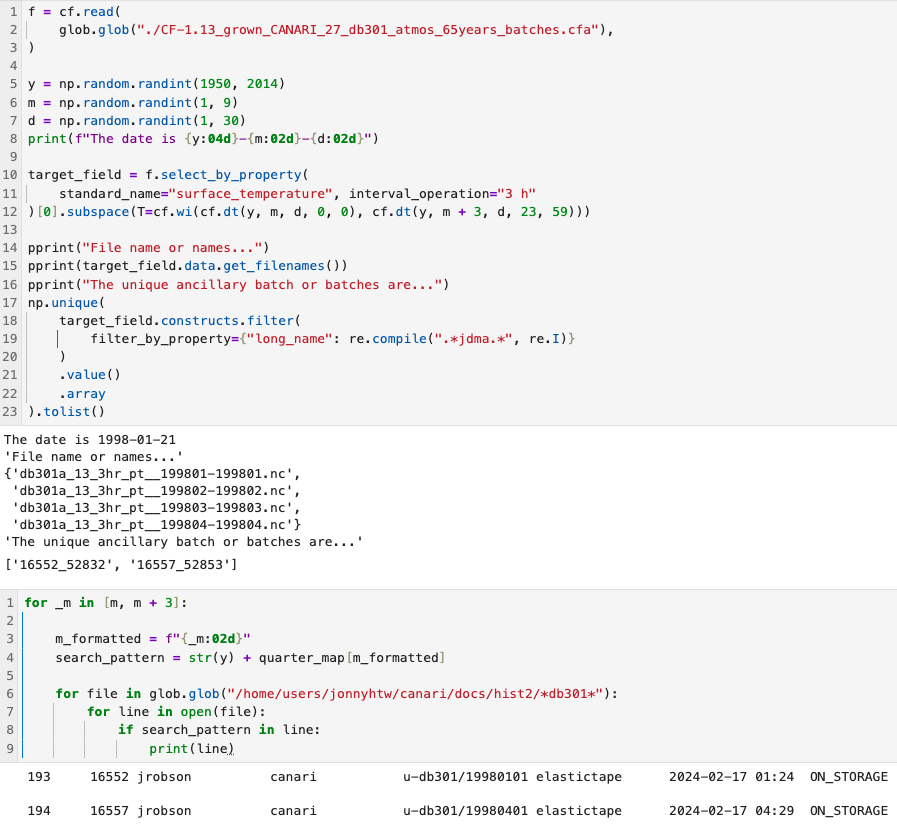
\includegraphics[width=\textwidth]{figures/CFAvalidation2}
    \caption{As for Figure \ref{fig:CFAvalidation} but over a period of 3 months, i.e. traversing two JDMA batches.}
    \label{fig:CFAvalidation2}
\end{figure} 

The code shown in Figure \ref{fig:CFAvalidation2} is slightly modified compared to Figure \ref{fig:CFAvalidation} in that the initial month selection is limited to January-September (inclusive) to ensure that when a 3-month `time delta' is added to the randomly chosen date, the year does not need to be changed to reflect this. This is purely for illustrative convenience and is not a limitation of the code.

Figure \ref{fig:CFAvalidation2} gives the randomly assigned initial date as 21/1/1998 and extends to 21/4/1998 giving the following list of files (the highlighted file indicates its presence in a different JDMA batch to the others):

\begin{enumerate}
    \item \texttt{\detokenize{db301a_13_3hr_pt__199801-199801.nc}}
    \item \texttt{\detokenize{db301a_13_3hr_pt__199802-199802.nc}}
    \item \texttt{\detokenize{db301a_13_3hr_pt__199803-199803.nc}}
    
    \item \colorbox{yellow}{\texttt{\detokenize{db301a_13_3hr_pt__199804-199804.nc}}}
\end{enumerate}

The unique JDMA batch numbers are given as 16552 and 16557. Again these agree with the `raw' \texttt{jdma batch} output.

For the external IDs, once again they agree (Figure \ref{fig:CFAvalidation2}).

\begin{itemize}
    
\item \texttt{jdma batch 16552|grep -i external
    External id  : 52832}

   \item  \texttt{jdma batch 16557|grep -i external
    External id  : 52853}



\end{itemize}






\section{Conclusions}\label{conc}

This work has expanded on previous work to catalogue the variables in the CANARI historical and SSP3-7.0 scenario ensembles. This has been done using the aggregation capabilities of the \texttt{cf} Python package \citep{hassell2017}, termed `CFA'.

This process involves three discrete steps; seeding, growth and arrangement. The first of these generates the template (i.e. `seed') for the first month of a reference simulation, the second grows it out to the length of the simulation inferring the already-standardised filenames, and the third assigns the correct tape archive `batch' numbers thus enabling later file discovery (`arrangement').

The work has been version controlled using Git and is broadly applicable to similarly-standardised datasets of arbitrary size. 

The largest time resource is taken up by the primary seeding step. This can be seen in Appendix \ref{bench} which shows that the generation of the seed file for the atmosphere realm of the historical scenario takes approximately 1~hour, the growth step take 16~minutes and arrangement 6~seconds.

That said, the seeding only needs to be run once for each data instance; e.g. atmosphere data for a particular climate scenario. In this case there was a small change to the diagnostic set in ensemble members 13-40 which necessitated the generation of a different seed, but this only adds $\mathcal{O}(1~\mathrm{hour})$ to the overall computation time since a new seed file must be created. 

These scripts -- although predicated on the CANARI ensemble and pre-formatted filenames -- could straightforwardly be edited and used by other large datasets. 






\appendices

\section{Benchmarking}\label{bench}

This section compares the time taken in each of the seed, grow and arrange steps for the atmosphere realm of \texttt{u-cy537}, the 13th member of the historical ensemble; see Table \ref{tab:runids}.

\subsection{Seed}\label{aseed}

Listing \ref{lst:seed}


\begin{center}
\begin{minipage}{\textwidth}
\begin{lstlisting}[
    basicstyle=\small\ttfamily,
    frame=single,caption={\texttt{seed.py}},
    backgroundcolor=\color{gray!5},
    breaklines=true,label={lst:seed},
    keepspaces=true,
    columns=fullflexible
]
time python seed.py --runid     cy537\ 
                    --member    13\
                    --realm     atmos\
                    --data_path $HOME/archive/CANARI/u-cy537/19500101T0000Z/\ 
                    --startyear 1950
\end{lstlisting}
\end{minipage}
\end{center}

\begin{table}[h]
    \centering
    \caption{Timings for arrange, historical, atmosphere, using the output from the \texttt{time} Linux command. The `real' time is the `Elapsed real time (in seconds)', `user' is `Total number of CPU-seconds that the process spent in user mode.' and `sys' is `Total number of CPU-seconds that the process spent in kernel mode.' where the definitions are from the \texttt{man time} Linux command.}
    \label{tab:seedtable}
    \begin{tabular}{l l}
        \hline
        Measure & time  \\
        \hline
         real   & 59~m~15~s  \\
        user   & 55~m~18~s  \\
        sys     & 2~m~37~s  \\ 
        \hline
    \end{tabular}
\end{table}










\subsection{Grow}

As for \S~\ref{aseed} for the growth step. Code usage in Listing \ref{lst:grow}.

\begin{center}
\begin{minipage}{\textwidth}
\begin{lstlisting}[
    basicstyle=\small\ttfamily,
    frame=single,caption={\texttt{grow.py}},
    backgroundcolor=\color{gray!5},label={lst:grow},
    breaklines=true,
    keepspaces=true,
    columns=fullflexible
]
time python grow.py --runid   cy537\ 
                    --member  13\
                    --realm   atmos\
                    --n_years 65
\end{lstlisting}
\end{minipage}
\end{center}

\begin{table}[h]
    \centering
    \caption{Timings for grow, historical, atmosphere, using the output from the \texttt{time} Linux command. The `real' time is the `Elapsed real time (in seconds)', `user' is `Total number of CPU-seconds that the process spent in user mode.' and `sys' is `Total number of CPU-seconds that the process spent in kernel mode.' where the definitions are from the \texttt{man time} Linux command.}
    \label{tab:growtable}
    \begin{tabular}{l l}
        \hline
        Measure & time  \\
        \hline
         real   & 16~m~16~s  \\
        user   & 15~m~16~s  \\
        sys     &  0~m~27~s  \\ 
        \hline
    \end{tabular}
\end{table}







\subsection{Arrange}

As for \S~\ref{aseed} for the arrange step. Code usage shown in Listing \ref{lst:arrange}.

\begin{center}
\begin{minipage}{\textwidth}
\begin{lstlisting}[
    basicstyle=\small\ttfamily,
    frame=single,label={lst:arrange}, caption={\texttt{arrange.py}},
    backgroundcolor=\color{gray!5},
    breaklines=true,
    keepspaces=true,
    columns=fullflexible
]
time python arrange.py --member   13\
                       --realm    atmos\
                       --n_years  65\
                       --scenario hist2
\end{lstlisting}
\end{minipage}
\end{center}

\begin{table}[h]
    \centering
    \caption{Timings for arrange, historical, atmosphere, using the output from the \texttt{time} Linux command. The `real' time is the `Elapsed real time (in seconds)', `user' is `Total number of CPU-seconds that the process spent in user mode.' and `sys' is `Total number of CPU-seconds that the process spent in kernel mode.' where the definitions are from the \texttt{man time} Linux command.}
    \label{tab:arrangetable}
    \begin{tabular}{l l}
        \hline
        Measure & time  \\
        \hline
         real   & 0~m~26~s \\
        user   &   0~m~25~s\\
        sys     &  0~m~2~s\\ 
        \hline
    \end{tabular}
\end{table} 
 


\subsection{Comparison of time taken in seed, grow and arrange steps}

Figure \ref{fig:pie} shows the `real' time taken as shown in Tables \ref{tab:seedtable}, \ref{tab:growtable} and \ref{tab:arrangetable}.

\begin{figure}[htbp]
    \centering
    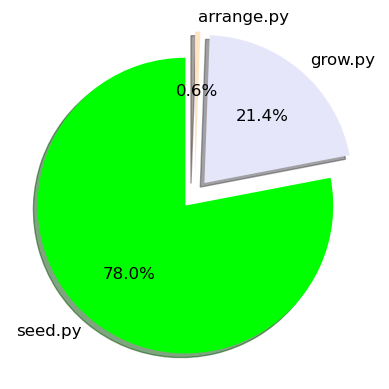
\includegraphics[width=0.8\textwidth]{figures/pie}
    \caption{Pie graph representation of the `real' times from Tables \ref{tab:seedtable}, \ref{tab:growtable} and \ref{tab:arrangetable}.}

    \label{fig:pie}
\end{figure} 



\section{Runtime instructions}

This section shows the command line `doc string' help available for the seed, grow and arrange steps.

\subsection{Seed}

Listing \ref{lst:aseed}.

\begin{minipage}{\textwidth}


\begin{lstlisting}[
    caption={Output of python seed.py -h},
    basicstyle=\small\ttfamily,
    frame=single,
    breaklines=true,label={lst:aseed},
    backgroundcolor=\color{gray!5},
    columns=fullflexible,
    keepspaces=true
]
usage: seed.py [-h] --runid RUNID --realm {atmos,ocean,ice} --member MEMBER [--testing {yes,no}] --startyear STARTYEAR
               --data_path DATA_PATH

Initializes CFA files from source data.

options:
  -h, --help            show this help message and exit
  --runid RUNID         Run ID in format letter-letter-number-number-number
  --realm {atmos,ocean,ice}
                        The climate realm
  --member, -m MEMBER   The ensemble member number
  --testing, -t {yes,no}
                        Is this a test run? (default: no)
  --startyear STARTYEAR
                        Starting year of the simulation.
  --data_path, -d DATA_PATH
                        Path to the source data directory

(cfa_env) sci-vm-01|Mon Mar 23|16:51:12 GMT|cfa_scripts|[main]> 
\end{lstlisting}
\end{minipage}


\subsection{Grow}

Listing \ref{lst:agrow}.

\begin{lstlisting}[
    caption={Output of python grow.py -h},
    basicstyle=\small\ttfamily,
    frame=single,
    breaklines=true,label={lst:agrow},
    backgroundcolor=\color{gray!5},
    columns=fullflexible,
    keepspaces=true
]
usage: grow.py [-h] --runid RUNID --realm {atmos,ocean,ice} --member MEMBER [--testing {yes,no}] --n_years N_YEARS

Appends data to existing CFA files.

options:
  -h, --help            show this help message and exit
  --runid RUNID
  --realm {atmos,ocean,ice}
  --member, -m MEMBER
  --testing, -t {yes,no}
                        Is this a test run? (default: no)
  --n_years, -ny N_YEARS

(cfa_env) sci-vm-01|Mon Mar 23|16:52:48 GMT|cfa_scripts|[main]> 
\end{lstlisting}


\subsection{Arrange}

Listing \ref{lst:aarrange}.

\begin{minipage}{\textwidth}
\begin{lstlisting}[
    caption={Output of python arrange.py -h},
    basicstyle=\small\ttfamily,
    frame=single,label={lst:aarrange},
    breaklines=true,
    backgroundcolor=\color{gray!5},
    columns=fullflexible,
    keepspaces=true
]
usage: arrange.py [-h] --member MEMBER --realm {atmos,ocean,ice} [--testing {yes,no}] --n_years N_YEARS --scenario {hist2,ssp370}

Adds in JDMA batch numbers.

options:
  -h, --help            show this help message and exit
  --member, -m MEMBER   Ensemble member.
  --realm {atmos,ocean,ice}
  --testing, -t {yes,no}
                        Is this a test run? (default: no)
  --n_years, -ny N_YEARS
  --scenario, -s {hist2,ssp370}

(cfa_env) sci-vm-01|Mon Mar 23|16:54:10 GMT|cfa_scripts|[main]> 
\end{lstlisting}
\end{minipage}


\section{Priority variables}


\subsection{Background}

The entirety of this report has dealt with the CF aggregration of the entire CANARI output as stored (currently, May 2026) on the JDMA system. For many applications however, only a subset of data is required and this is referred to as the `priority variables' -- PVs --  set. Detailed information regarding the variables themselves can be found on the relevant \href{https://ncas-cms.github.io/canari/#priority-and-derived-output-on-jasmin-canari-group-workspace}{NCAS-CMS GitHub page}.

\subsection{Algorithm}

For the priority variables, all data is accessible `live' on the `canari' Group Workspace on JASMIN at `/gws/ssde/j25b/canari/large-ensemble/priority-variables`. In addition, the PVs are pre-separated into single variable files, for example (see Figure \ref{fig:ATMOCNCICE}):

\begin{itemize}

    \item \texttt{\detokenize{cv575a_1_1hr_m01s05i216.nc}}, for the atmosphere.
        \begin{itemize}
    \item Surface temperature after timestep [\degree K], details of variables can be found on the \href{https://reference.metoffice.gov.uk/um/stash}{UM STASH browser}.
    % \item For example see Figure \ref{fig:ATM}.
\end{itemize}
    \item \texttt{\detokenize{cv575o_1_day__grid_T_tos.nc}}, for the ocean.
        \begin{itemize}
            \item Sea surface temperature [\degree C].
            % \item For example Figure \ref{fig:OCN}
            \end{itemize}
    \item \texttt{\detokenize{cv575i_1_day_aice.nc}}, for the sea ice.
        \begin{itemize}
            \item Ice area (aggregate) $ \in [0, 1]$.
            % \item For example Figure \ref{fig:CICE}

            \end{itemize}

\end{itemize}


Because of the availability of the PVs on disk, the process for obtaining the CFA files representing each realm is greatly simplified and is performed by a single Python script, \texttt{priority-variables.py}. This script reads in all the data for each member of the historical and SSP3-7.0 ensembles and writes out one CFA files for each variable/scenario/member combination. The \texttt{priority-variables} Python script which performs this is illustrated using \texttt{PlantUML} in Figure \ref{fig:priority-variables}.


\begin{figure}
    \centering
    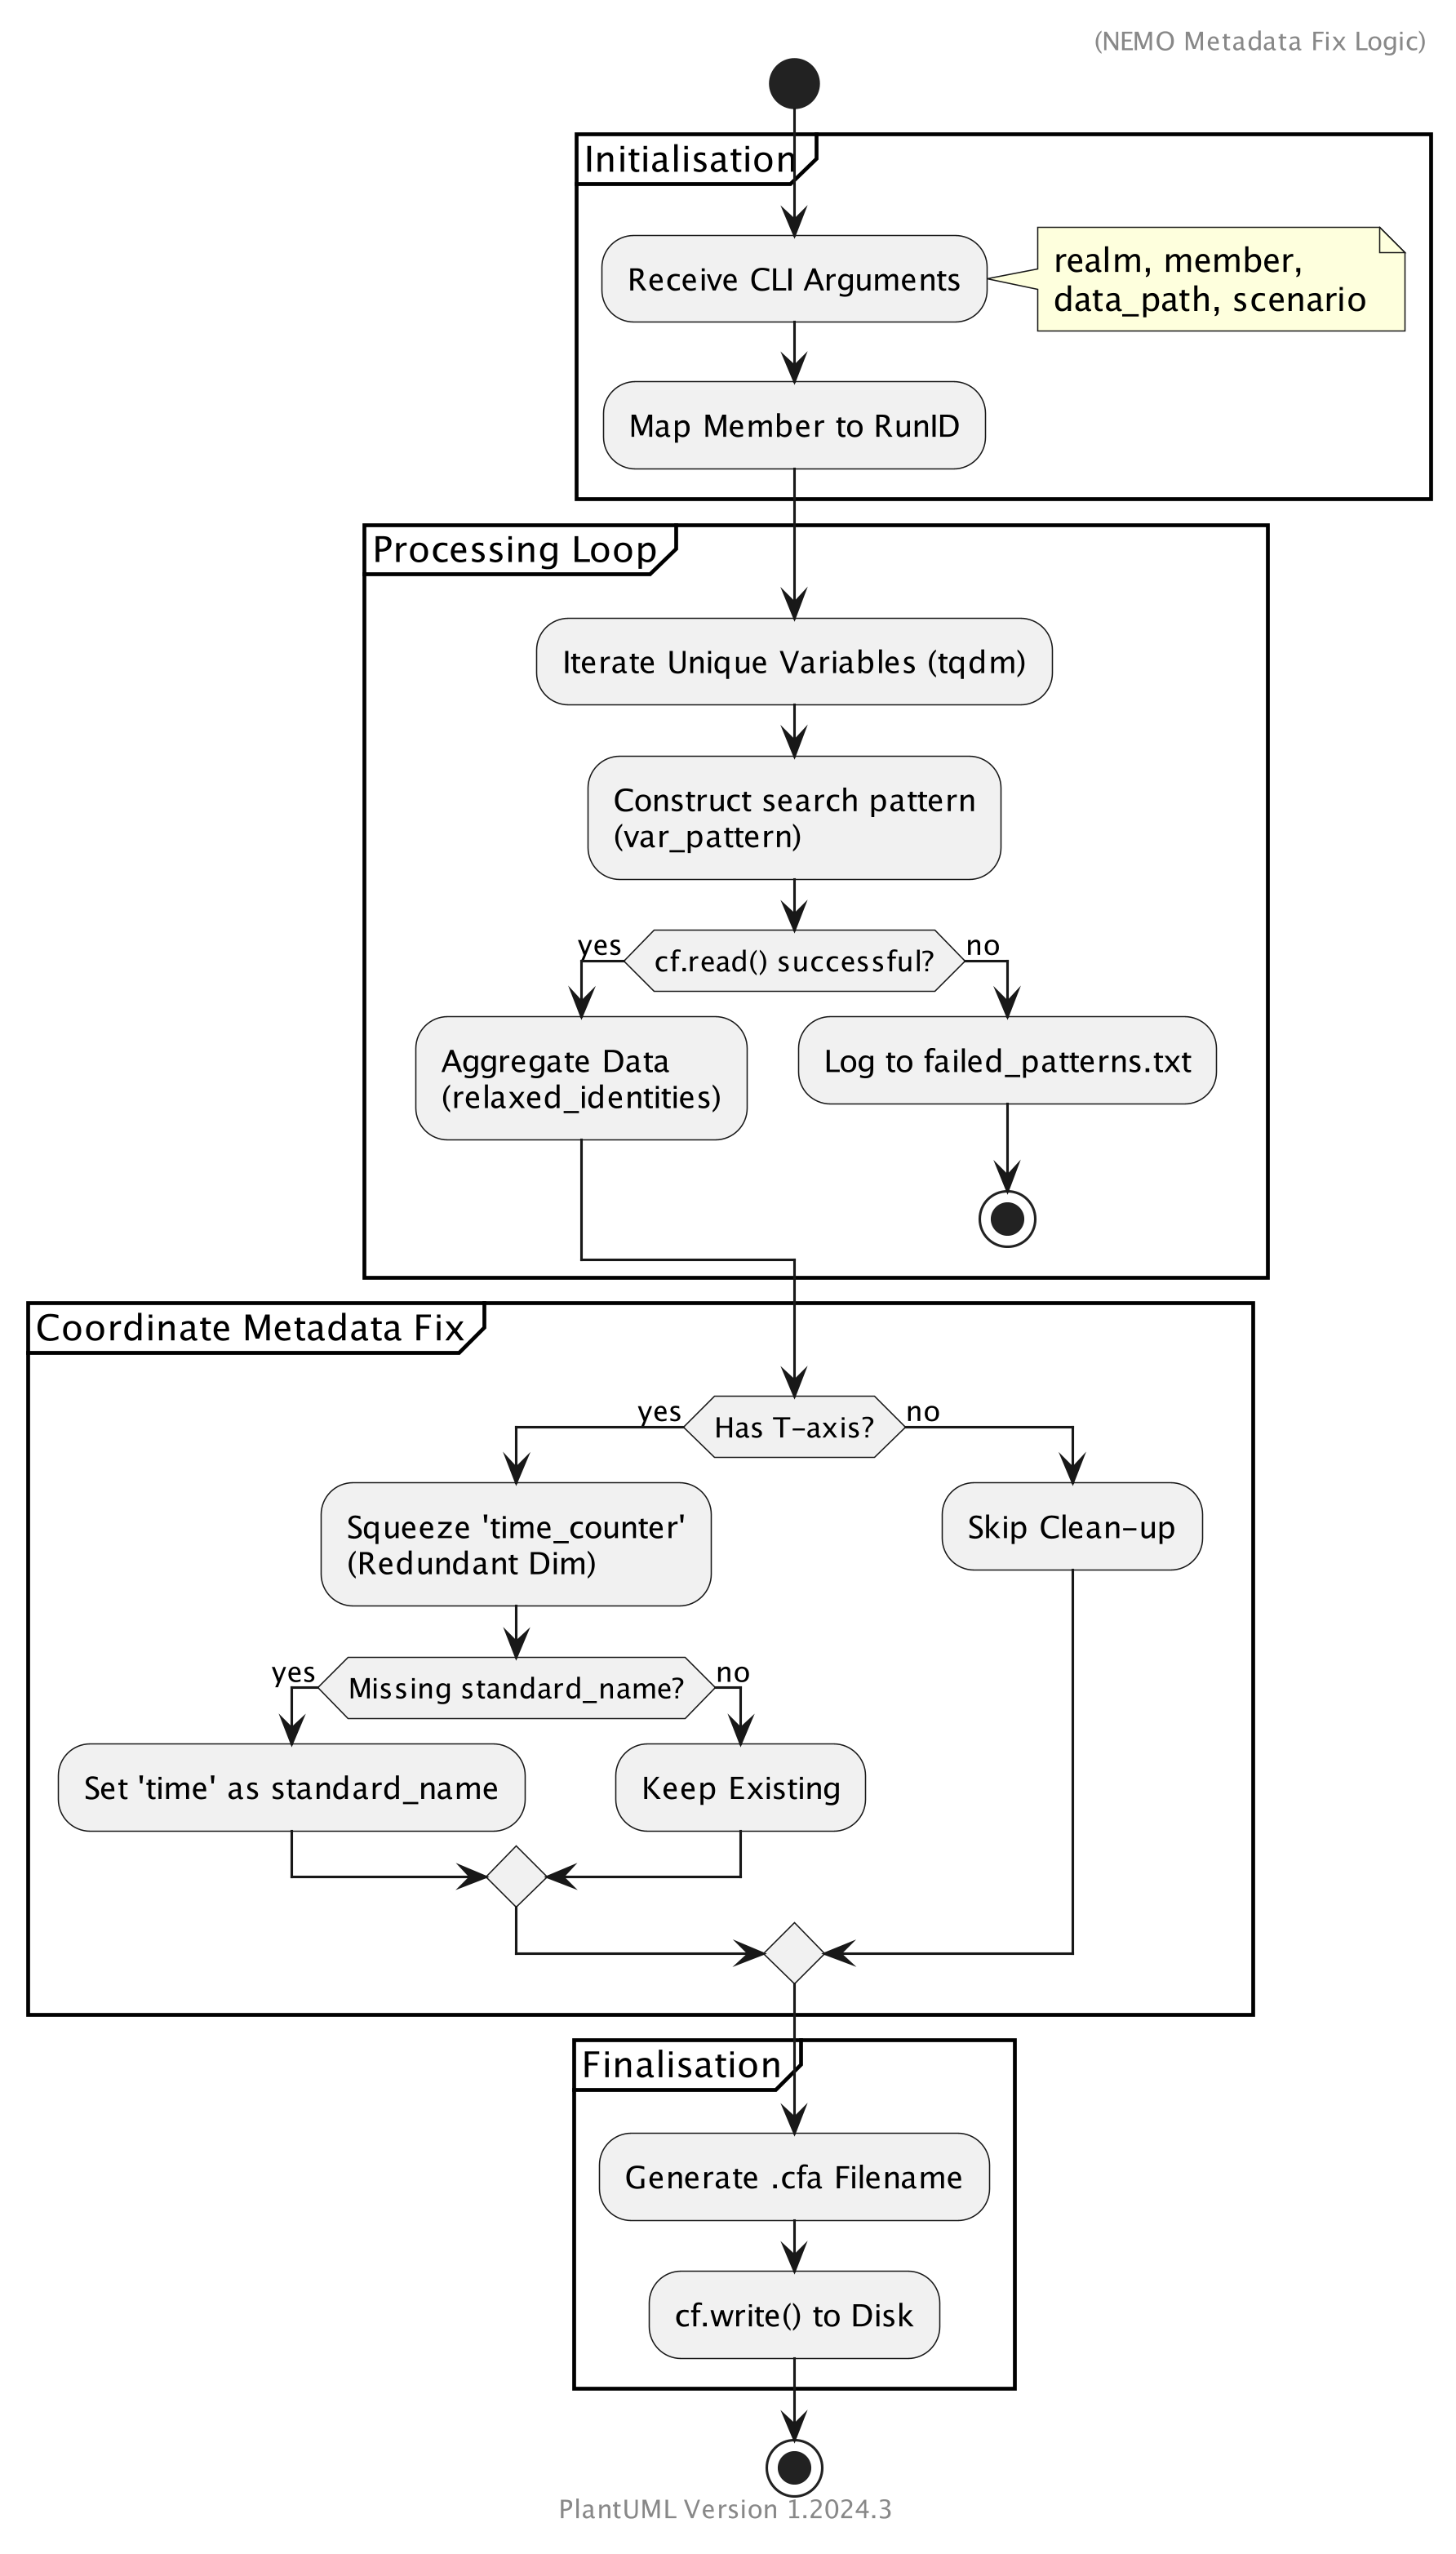
\includegraphics[width=0.8\textwidth]{figures/priority-variables.png}
    \caption{Algorithm for the \texttt{priority-files.py} file, Figure prepared using \texttt{PlantUML}. }
    \label{fig:priority-variables}
\end{figure}

\begin{minipage}{\textwidth}
\begin{lstlisting}[
    caption={Output of python priority-variables.py {-}{-}help},
    basicstyle=\small\ttfamily,
    frame=single,label={lst:priority-variables},
    breaklines=true,
    backgroundcolor=\color{gray!5},
    columns=fullflexible,
    keepspaces=true
]
python priority-variables.py --help
Usage: priority-variables.py [OPTIONS]

  Create seed CFA file for CANARI priority variables.

Options:
  --realm [ATM|OCN|CICE]     The climate realm  [required]
  --verbose INTEGER RANGE    Verbosity level of cf.read  [-1<=x<=3]
  --scenario [HIST2|SSP370]  The scenario  [required]
  -m, --member INTEGER       The ensemble member number  [required]
  -d, --data_path PATH       Path to the source data directory  [required]
  --help                     Show this message and exit.
(cfa_env) sci-vm-01|Wed May 27|15:44:32 BST|priority-variables|[priority-variables]>
\end{lstlisting}
\end{minipage}


\begin{figure}[htbp]
    \centering
    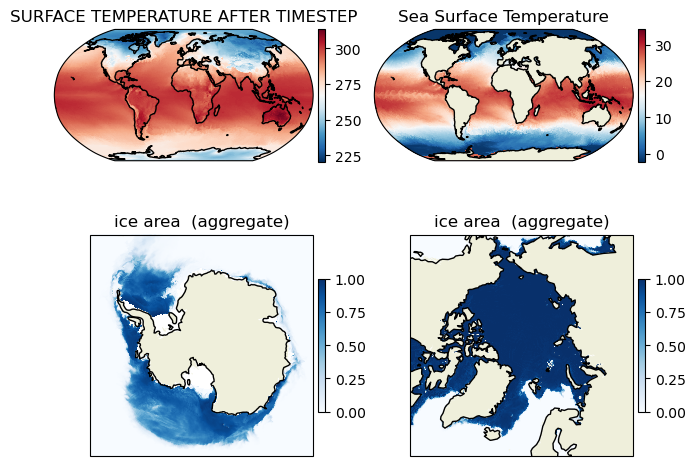
\includegraphics[width=0.8\textwidth]{figures/ATMOCNCICE}
    \caption{Example surface air temperature after timestep (in Kelvin), sea surface temperature (in Celsius), and sea ice area (aggregate) from ensemble member 1 of the historical ensemble.}
    \label{fig:ATMOCNCICE}
\end{figure} 

The code for generating Figure \ref{fig:ATMOCNCICE} is shown in Listing \ref{lst:ATMOCNCICE}.


\clearpage



\begin{lstlisting}[
    caption={Code to generate Figure \ref{fig:ATMOCNCICE}.}, % Added backslash here
    basicstyle=\small\ttfamily,
    label={lst:ATMOCNCICE},
    frame=single,
    breaklines=true,
    backgroundcolor=\color{gray!5},
    columns=fullflexible,
    keepspaces=true
]
import matplotlib.pyplot as plt
import cartopy.crs as ccrs
import cartopy.feature as cfeature
import cf

files = [
    "./CF-1.13_seed_CANARI_1_cv575_ATM_1_mon_m01s00i024_3.cfa",
    "./CF-1.13_seed_CANARI_1_cv575_OCN_day__grid_T_tos.cfa",
    "CF-1.13_seed_CANARI_1_cv575_CICE_day_aice.cfa",
] + [
    "CF-1.13_seed_CANARI_1_cv575_CICE_day_aice.cfa",
]

fig, axes = plt.subplots(
    nrows=2,
    ncols=2,
    layout="constrained",
)

if len(files) == 1:
    axes = [axes]
else:
    axes = axes.flatten()

cmaps = ["RdBu_r"] * 2 + ["Blues"] * 2

for i in range(len(files)):
    old_ax = axes[i]
    pos = old_ax.get_subplotspec()
    old_ax.remove()

    if i < 2:
        proj = ccrs.Robinson()
    elif i == 2:
        proj = ccrs.SouthPolarStereo()
    elif i == 3:
        proj = ccrs.NorthPolarStereo()

    ax = fig.add_subplot(pos, projection=proj)

    fields = cf.read(files[i])
    f = fields[0][0]  

    mesh = ax.pcolormesh(
        f.construct("X").data.array,
        f.construct("Y").data.array,
        f.data.array.squeeze(),
        transform=ccrs.PlateCarree(),
        shading="auto",
        cmap=cmaps[i],
        zorder=0,
    )

    ax.coastlines(resolution="110m", linewidth=1)

    if i == 2:
        ax.set_extent([-180, 180, -90 * (i == 2), -60 * (i == 2)], ccrs.PlateCarree())
    elif i == 3:
        ax.set_extent([-180, 180, 60, 90], ccrs.PlateCarree())
    else:
        ax.set_global()

    if i > 0:
        ax.add_feature(cfeature.LAND, zorder=1)

    plt.colorbar(mesh, ax=ax, orientation="vertical", pad=0.02, shrink=0.6)

    title_text = getattr(f, "long_name", f"File {i}")
    ax.set_title(title_text)

plt.show();

\end{lstlisting}



\clearpage

\subsection{Discovery and generation of single-variable files}

The full CANARI data set is held on the JDMA system -- see page \pageref{jdma} -- but to retrieve individual variables there is a 2 step process: 

\begin{enumerate}
    \item Retrieve monthly data from JDMA for the years(s) required (see Figure \ref{fig:jdma_get_monthly}).
    \item Extract the required data and write to single-variable files (see Figure \ref{fig:get-yearly}).
\end{enumerate}

\subsubsection{Retrieval}

Figure \ref{fig:jdma_get_monthly} shows this graphically and Listing \ref{lst:jdma_get_monthly} gives the code implementation.


\begin{figure}
    \centering
    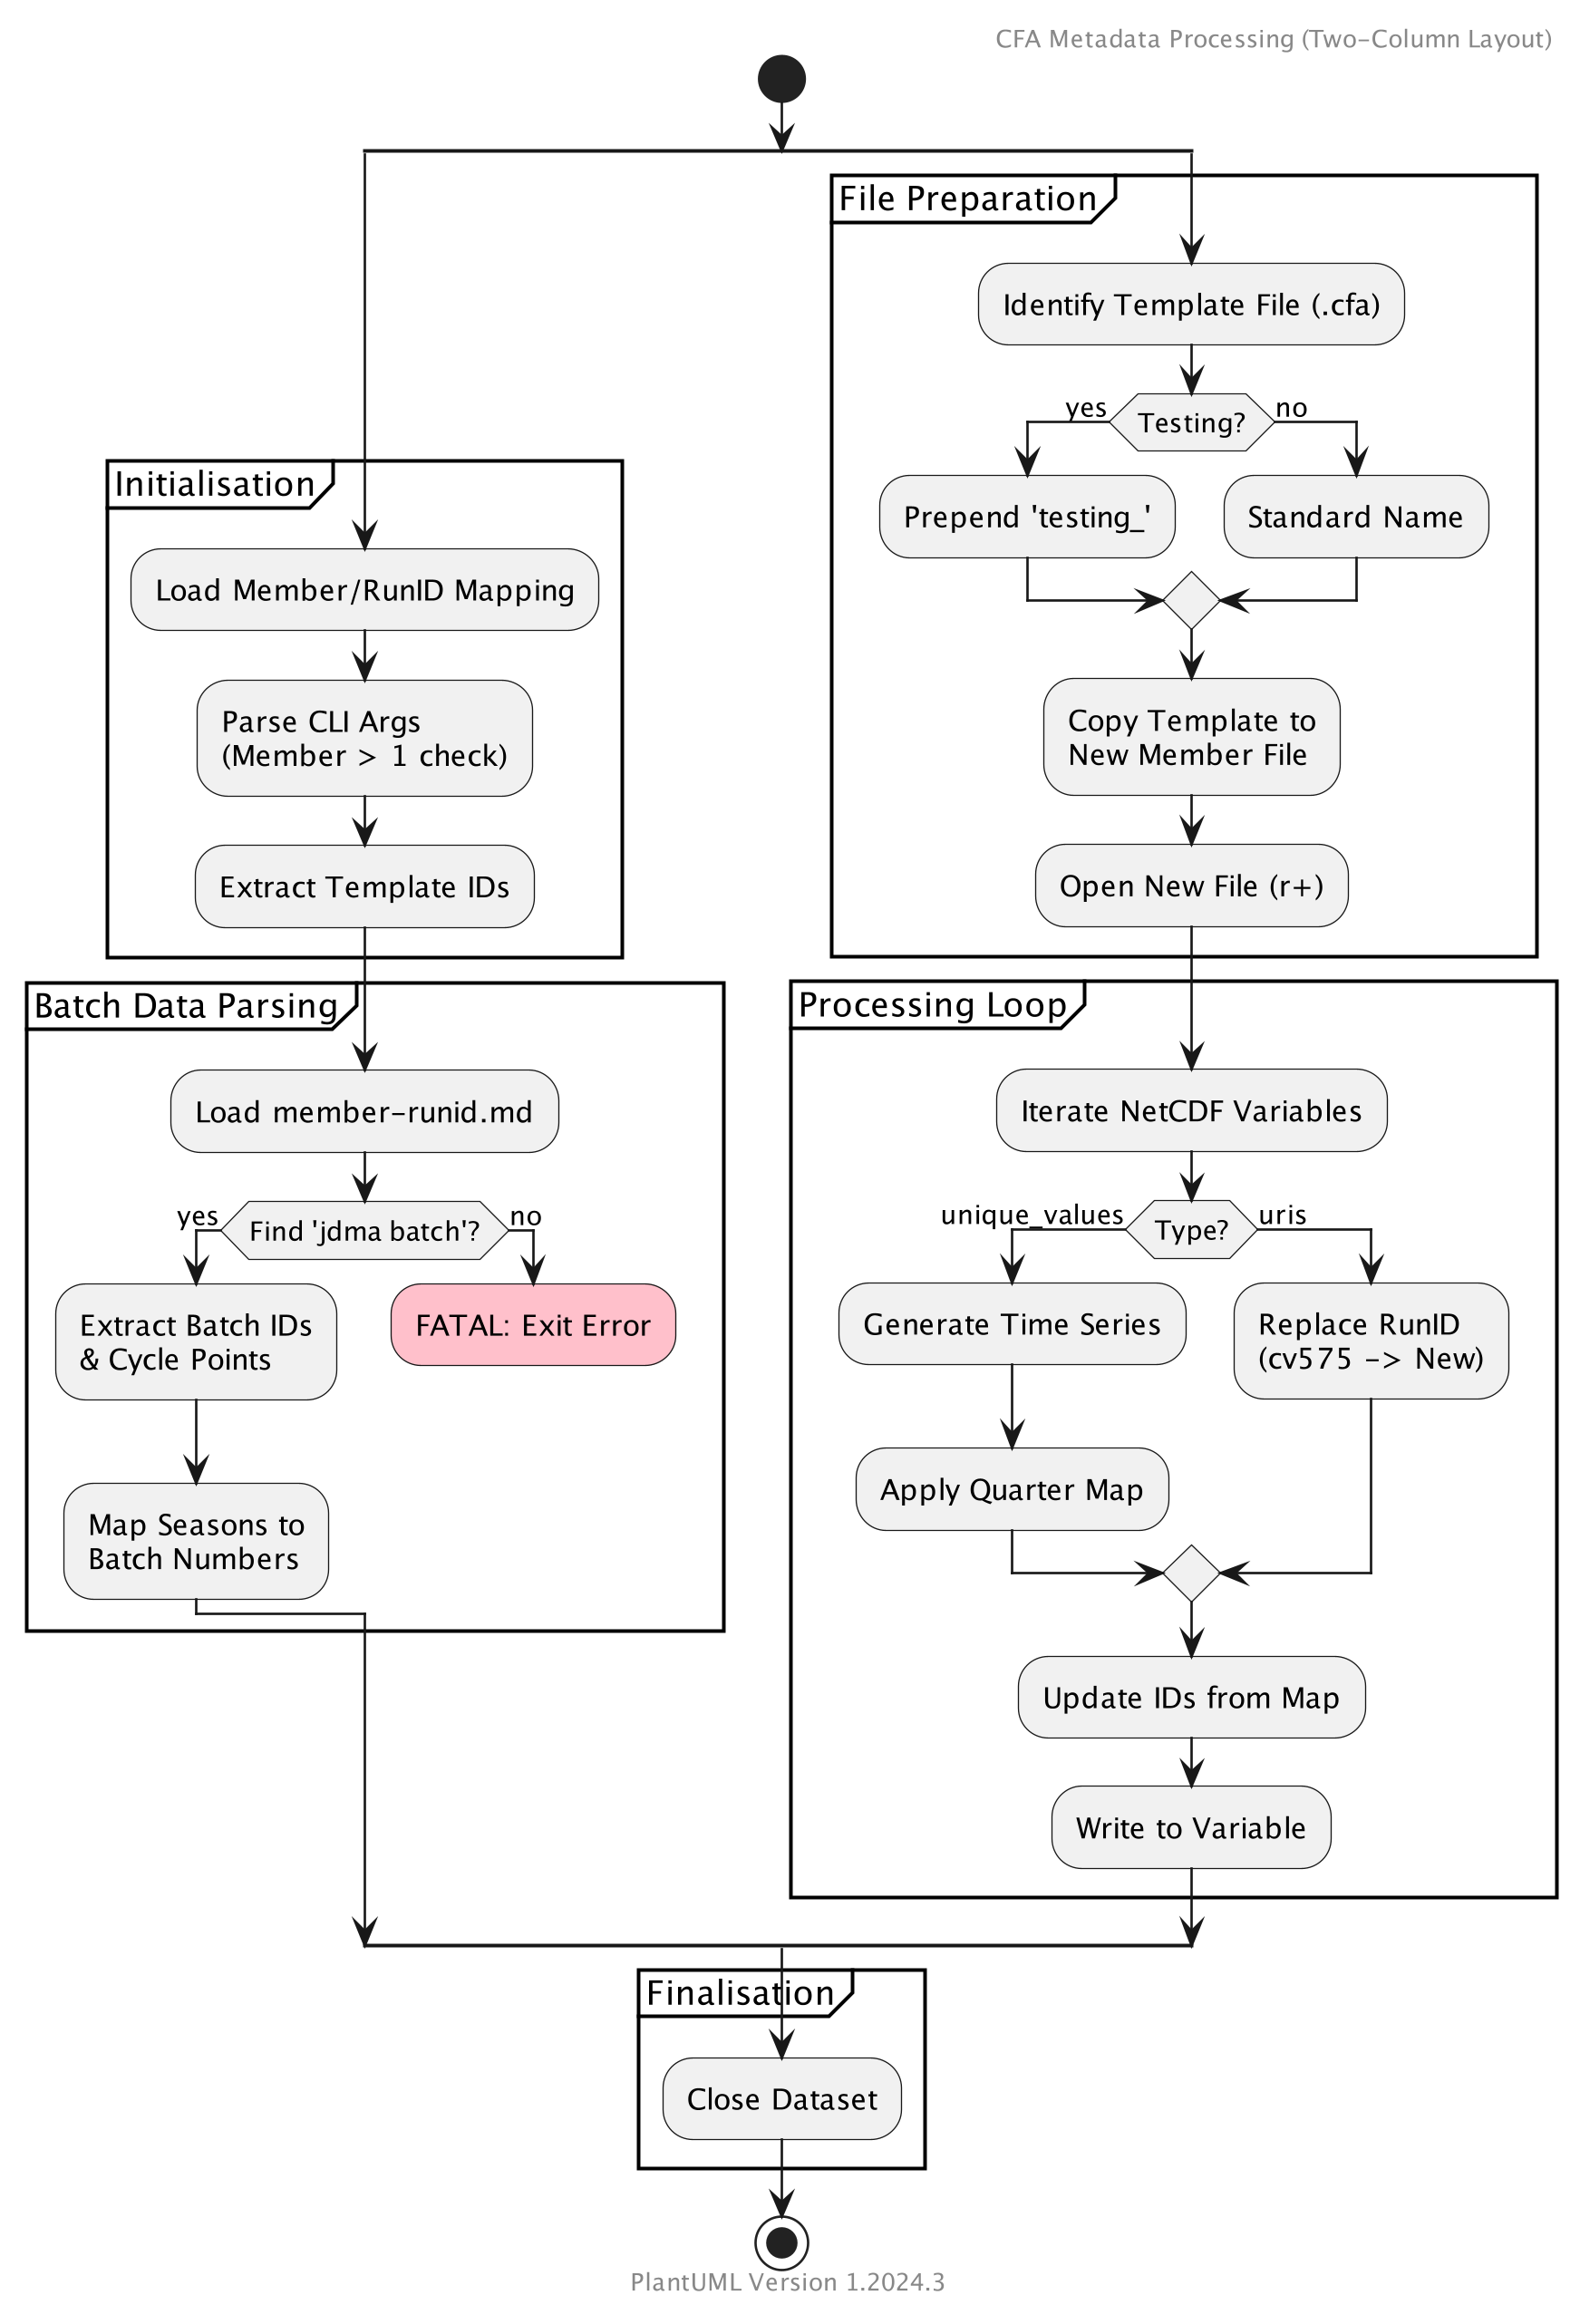
\includegraphics[width=0.8\textwidth]{figures/jdma_get_monthly.png}
    \caption{Algorithm for the \texttt{\detokenize{jdma_get_monthly.py}} file, Figure prepared using \texttt{PlantUML}. }
    \label{fig:jdma_get_monthly}
\end{figure} 

\begin{lstlisting}[
    caption={Output of python jdma\_get\_monthly.py {-}{-}help}, % Added backslash here
    label={lst:jdma_get_monthly},
    basicstyle=\small\ttfamily,
    frame=single,
    breaklines=true,
    backgroundcolor=\color{gray!5},
    columns=fullflexible,
    keepspaces=true
]
> python jdma_get_monthly.py --help
usage: jdma_get_monthly.py [-h] [--start START] [--end END] [--cycle CYCLE] [--filelist] [--ens ENS] suite

positional arguments:
  suite          Suite ID to extract data from

options:
  -h, --help     show this help message and exit
  --start START  Year from which to start extracting data from
  --end END      Year to extract data up to (included)
  --cycle CYCLE  Cycle (YYYYMM) for which to extract data for. Cannot be used in combination with --start/--end 
  --filelist     Create file(s) containing a list of files that would be extracted
  --ens ENS      Ensemble number of suite
(cfa_env) sci-vm-01|Tue May 26|15:27:35 BST|fix_corrupted|[priority-variables]>
\end{lstlisting}

\clearpage

\subsubsection{Extraction to yearly}


Figure \ref{fig:get-yearly} shows this graphically and Listing \ref{lst:get-yearly} gives the code implementation.


\begin{figure}[H]
    \centering
    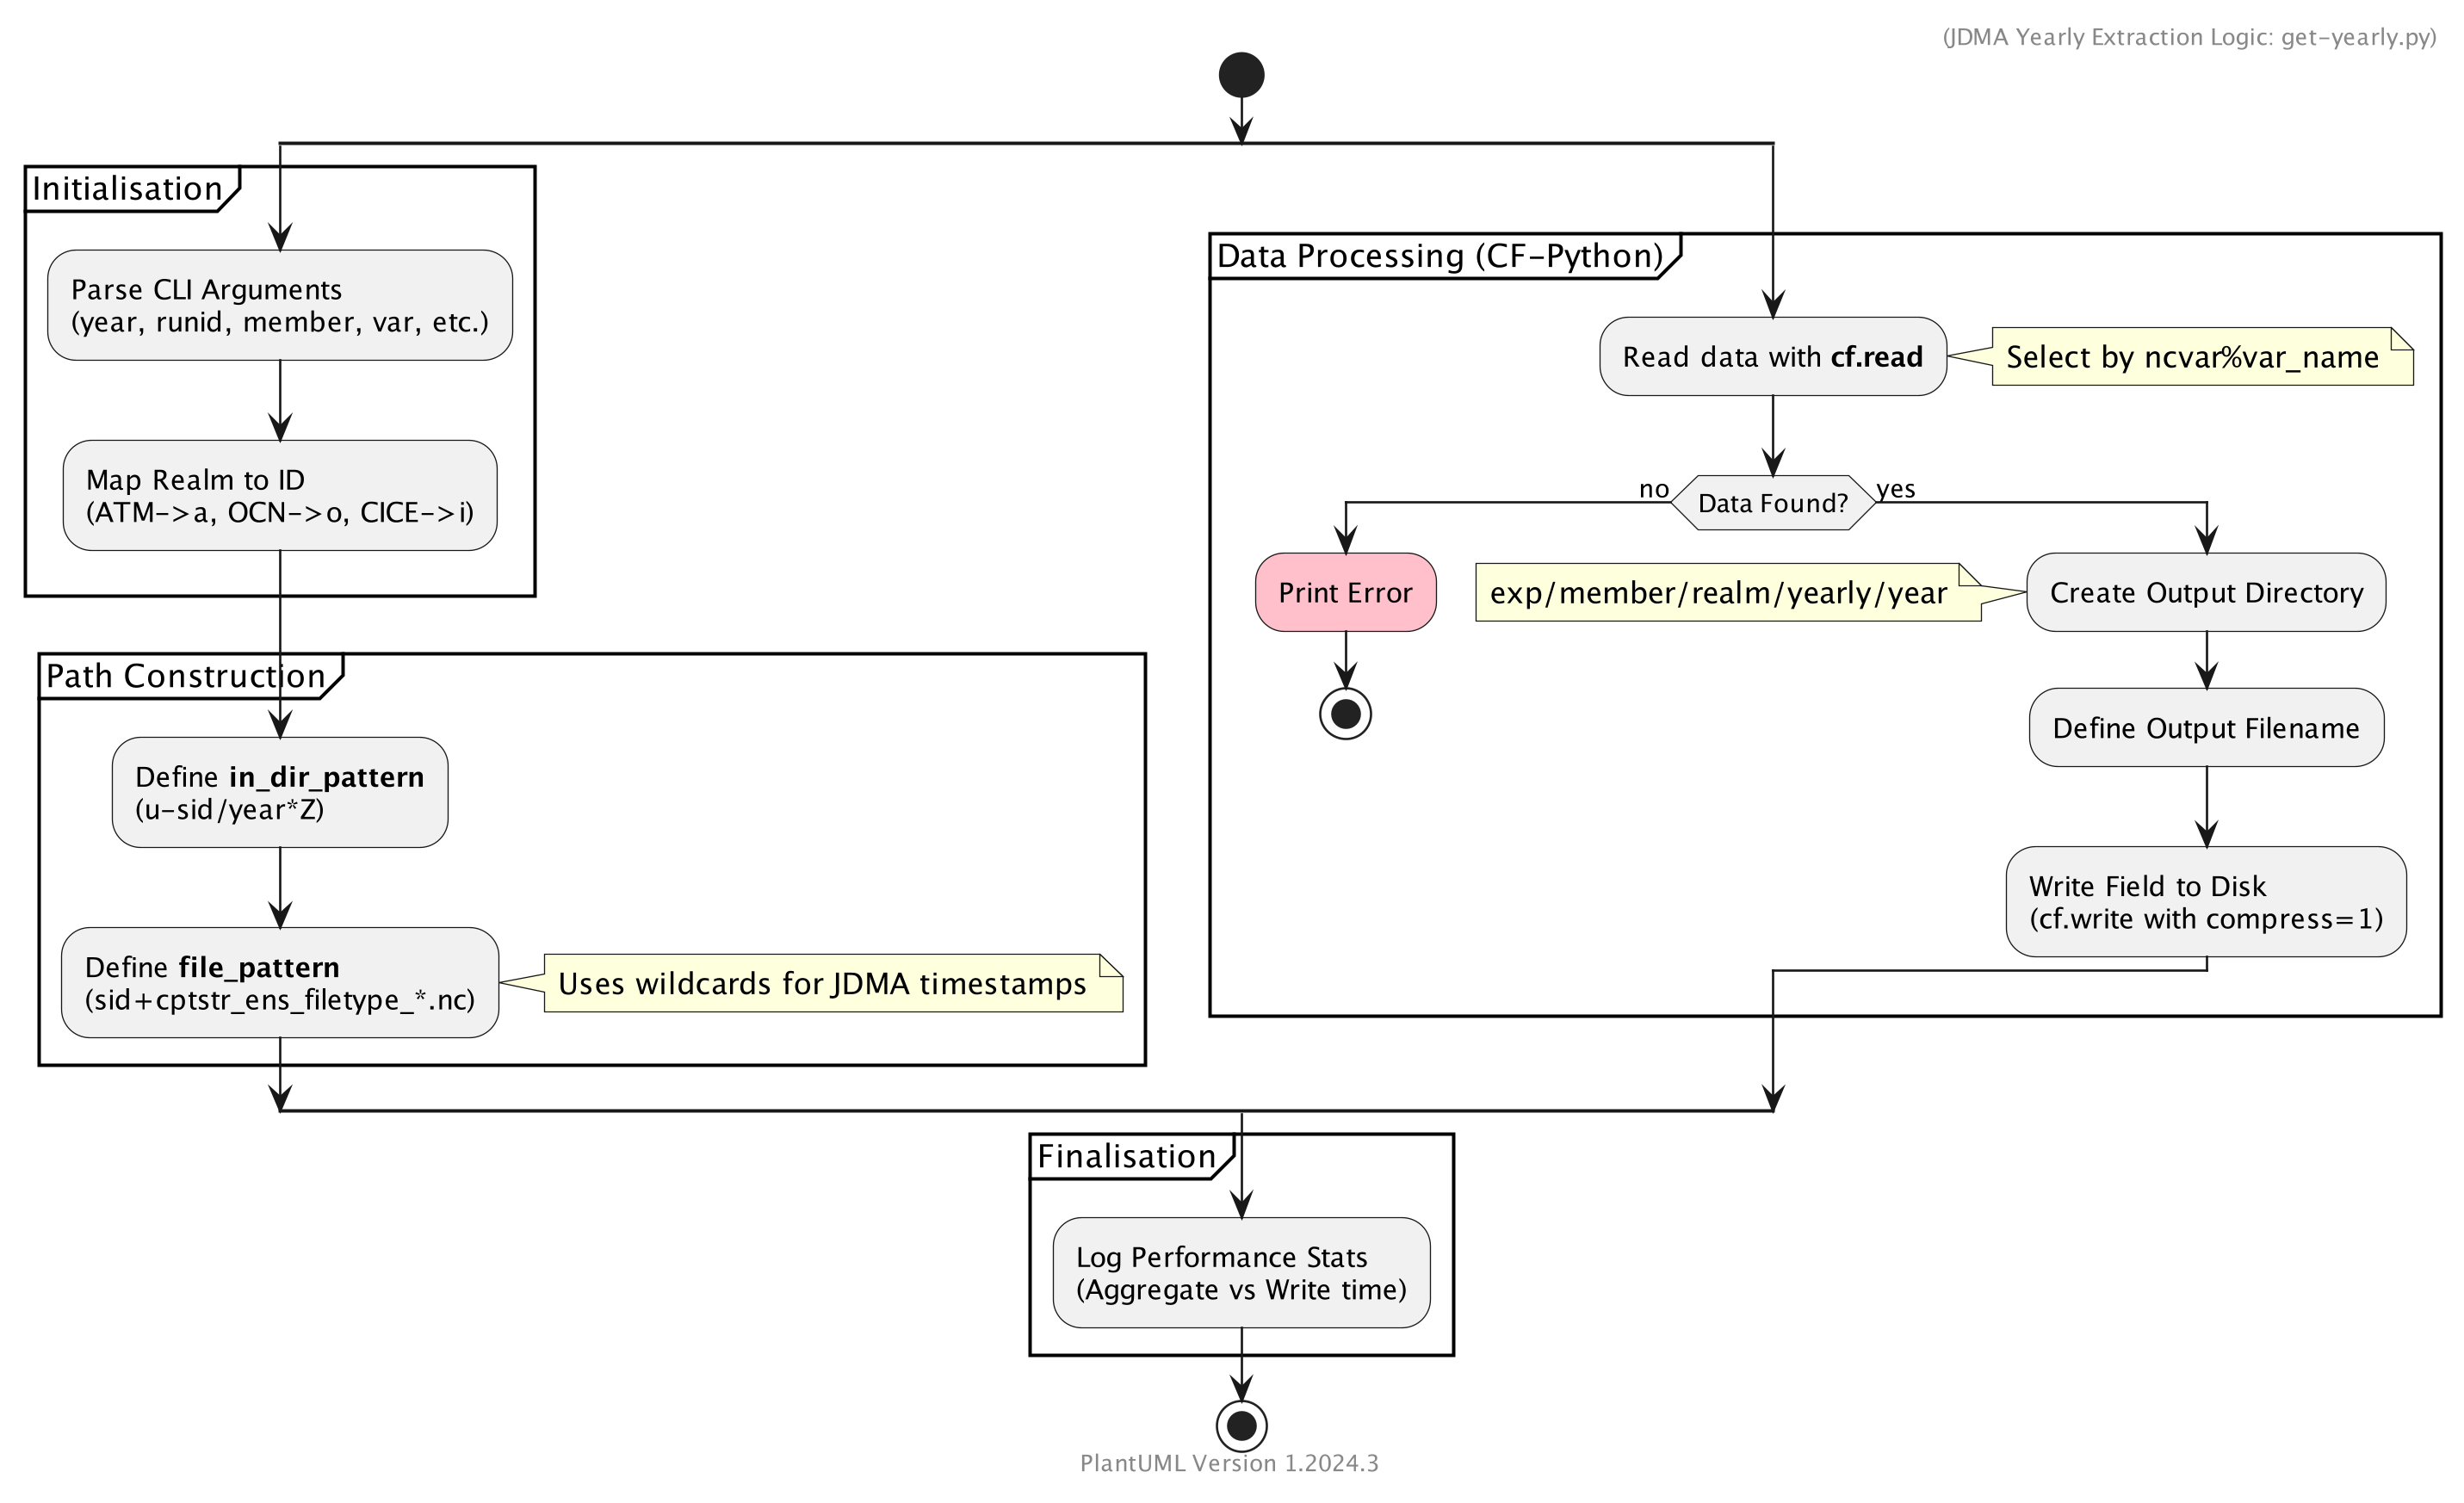
\includegraphics[width=0.8\textwidth]{figures/get-yearly.png}
    \caption{Algorithm for the \texttt{\detokenize{get-yearly.py}} file, Figure prepared using \texttt{PlantUML}. }
    \label{fig:get-yearly}
\end{figure} 



\begin{lstlisting}[
    caption={Output of python jget-yearly.py {-}{-}help}, % Added backslash here
    basicstyle=\small\ttfamily,
    label={lst:get-yearly},
    frame=single,
    breaklines=true,
    backgroundcolor=\color{gray!5},
    columns=fullflexible,
    keepspaces=true
]
> python get-yearly.py --help
usage: get-yearly.py [-h] --year YEAR --runid RUNID --member MEMBER --scenario SCENARIO --realm {ATM,OCN,CICE}
                     --filetype FILETYPE --var VAR

Extract single-year variables from JDMA-retrieved data.

options:
  -h, --help            show this help message and exit
  --year YEAR           Year to process (e.g. 1975)
  --runid RUNID         Run ID without the u- prefix (e.g. cz649)
  --member MEMBER       Ensemble member number
  --scenario SCENARIO   Scenario (e.g. HIST2)
  --realm {ATM,OCN,CICE}
                        Realm
  --filetype FILETYPE   Type (e.g. mon__diaptr)
  --var VAR             Var name (e.g. zotematl)

\end{lstlisting}



\clearpage



\subsection{Validation of corrupt priority-variable files}

Figure \ref{fig:validate-files} shows the validation process graphically and Listing \ref{lst:validate} shows the code implementation.

\begin{figure}
    \centering
    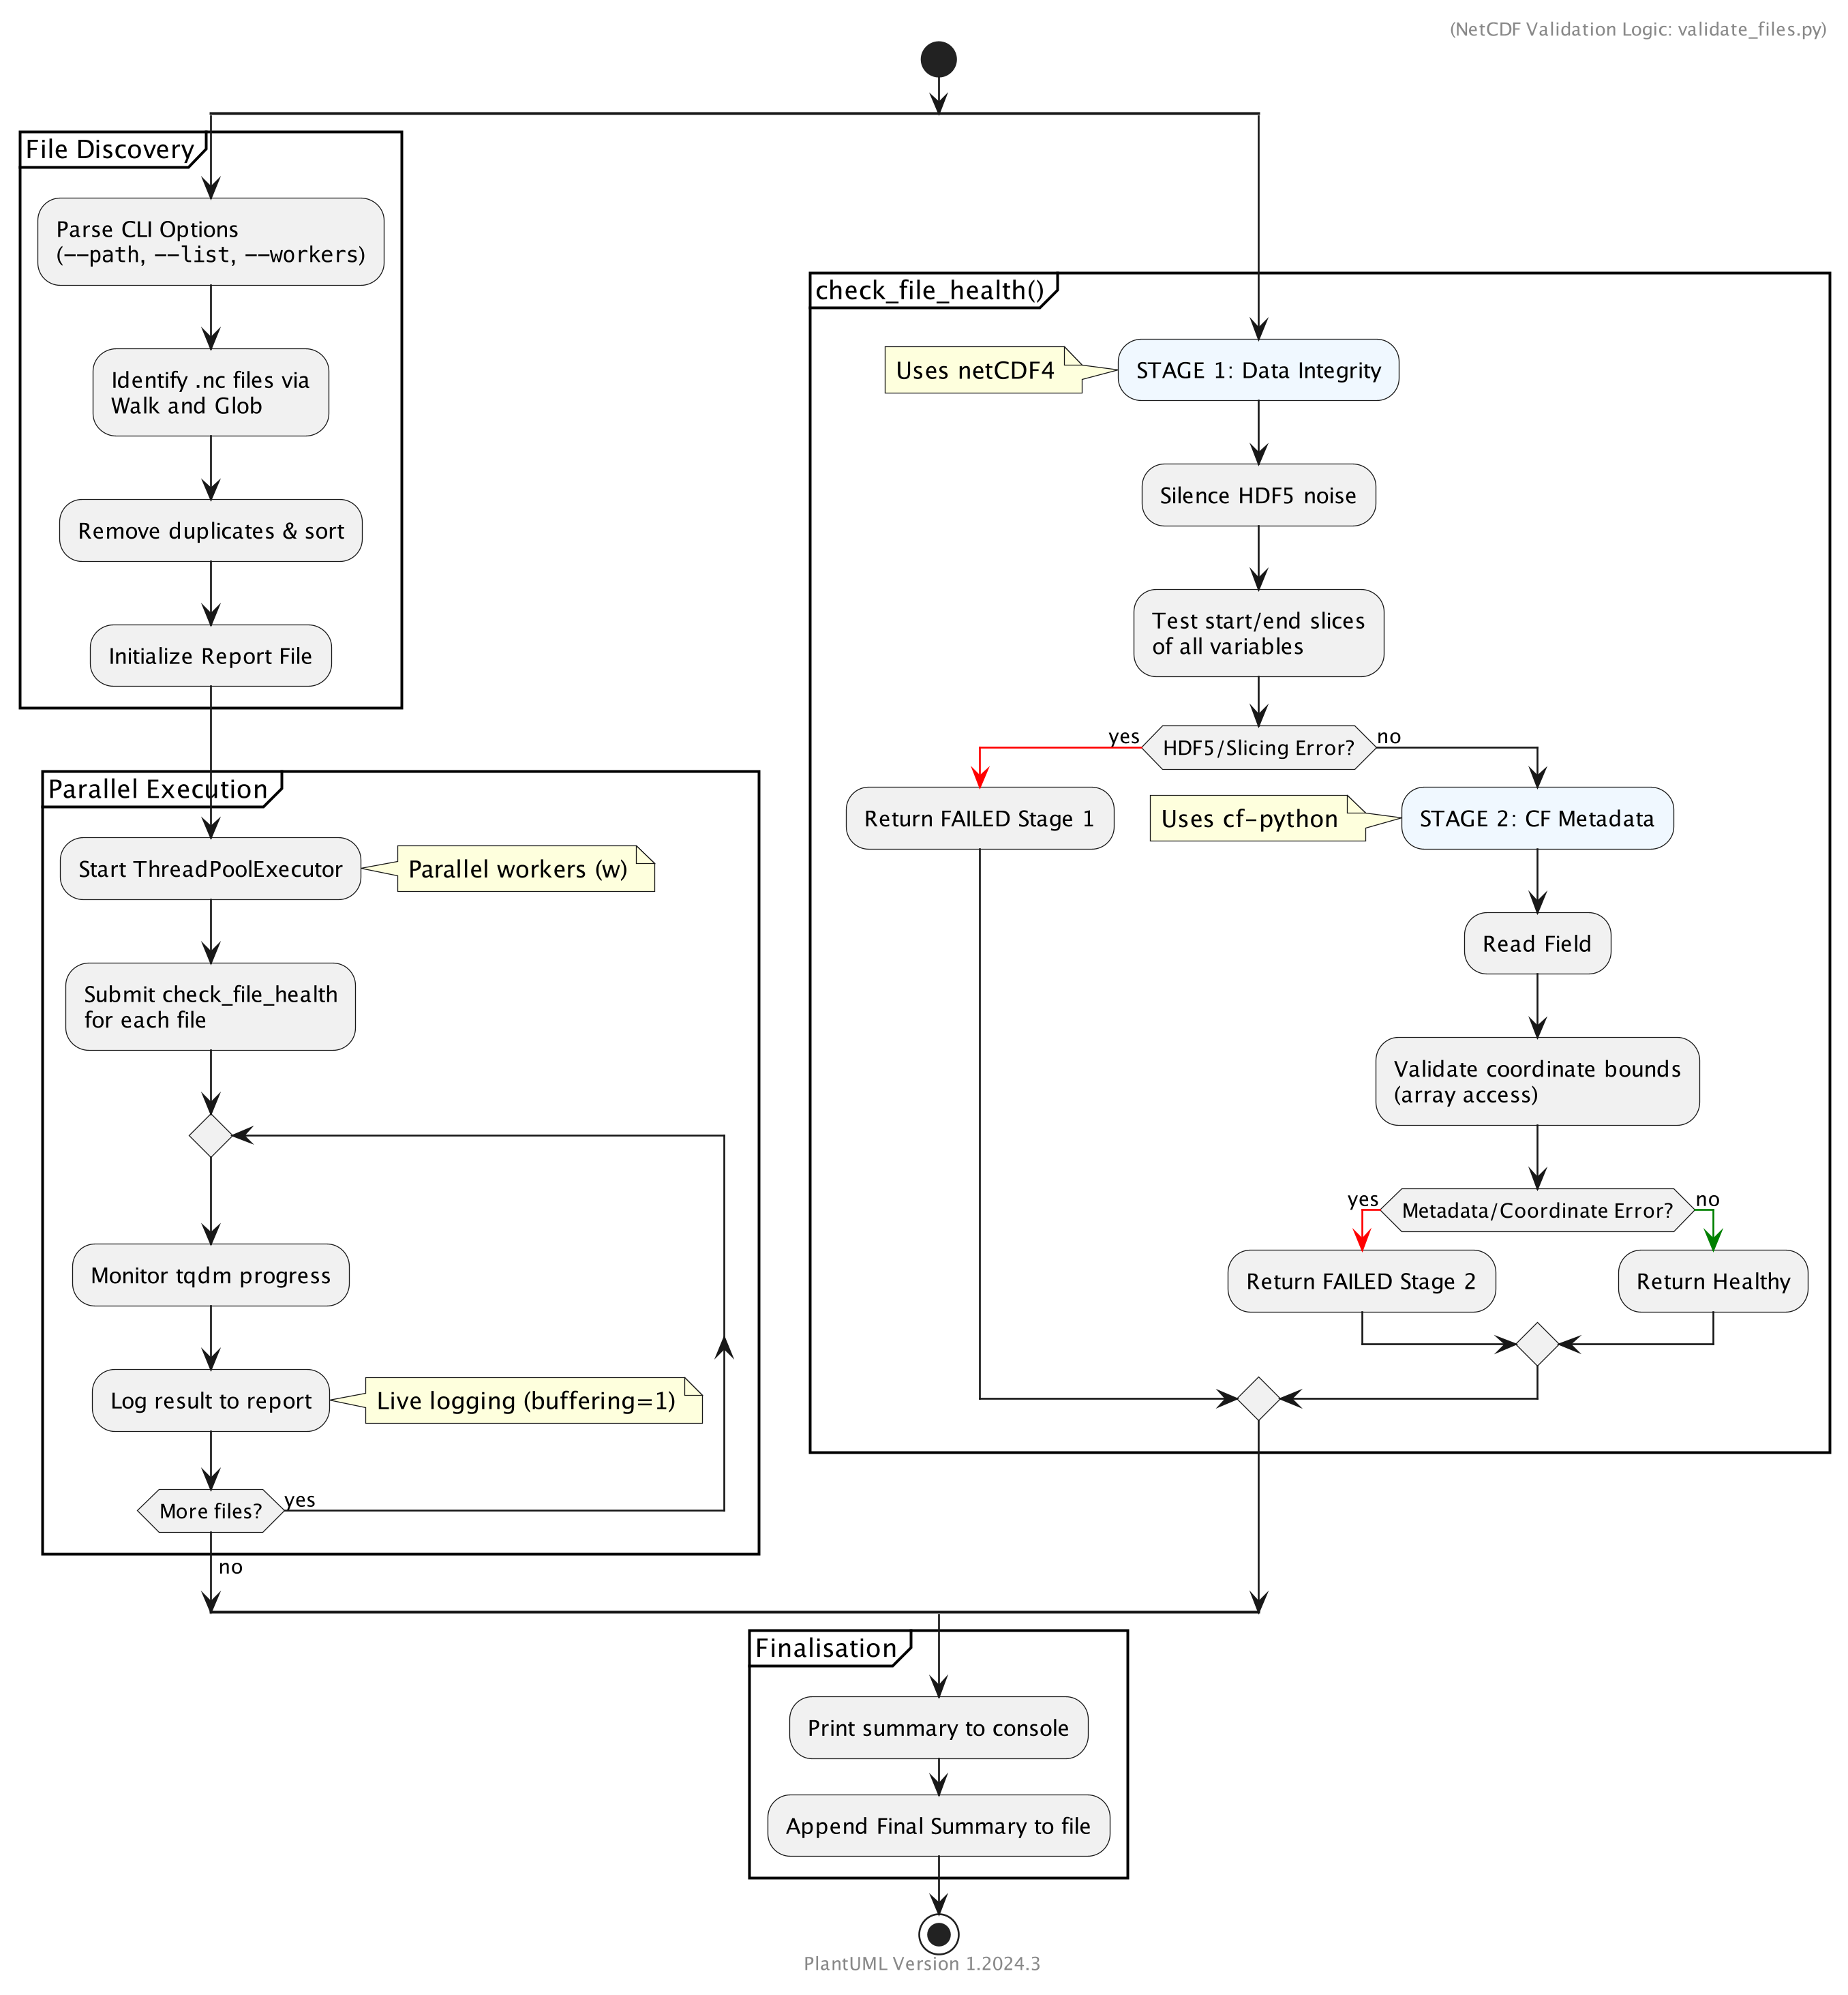
\includegraphics[width=0.8\textwidth]{figures/validate.png}
    \caption{Algorithm for the \texttt{\detokenize{validate-files.py}} file, Figure prepared using \texttt{PlantUML}. }
    \label{fig:validate-files}
\end{figure} 




\begin{lstlisting}[
    caption={Output of python validate-files.py {-}{-}help}, % Added backslash here
    basicstyle=\small\ttfamily,
    label={lst:validate},
    frame=single,
    breaklines=true,
    backgroundcolor=\color{gray!5},
    columns=fullflexible,
    keepspaces=true
]
> python validate-files.py  --help
Usage: validate-files.py [OPTIONS]

  Scan NetCDF files and generate a full Health Report (Live Logging).

Options:
  -p, --path TEXT        Path to scan.
  -l, --list PATH        Text file with paths.
  -w, --workers INTEGER  Number of parallel workers.
  -o, --out TEXT         Output report file.
  --help                 Show this message and exit.
(cfa_env) sci-vm-01|Tue May 26|16:02:45 BST|fix_corrupted|[priority-variables]>
\end{lstlisting}

The validation process is twofold; the checking of the presence of coordinate bounds, and the fidelity of the first and last slices of each diagnostic. The choice of these two tests was heuristic in the sense that there are many different tests that could be performed to assess the quality of model data but these tests were found sufficient to detect -- and subsequently fix -- all corrupt files.

Note that to enable corrupt-file discovery the \texttt{priority-variables.py} script shown in Figure \ref{fig:priority-variables} and Listing \ref{lst:priority-variables} enables the writing of Python `glob' strings which cause the CFA generation process to fail.  These lists can then be used to `home in' on specific broken files.




\clearpage

\bibliographystyle{plainnat} 
\bibliography{bib} 



\end{document}
